\documentclass[mathserif,18pt,xcolor=table]{beamer}
\usepackage{amsmath}
\usepackage{amssymb}
\usepackage{bbm}
\usepackage{ulem}
\usepackage{feynmp-auto}
\usepackage{slashed}
\usepackage{graphicx}
\usepackage{textpos}
\usepackage{listings}
\usepackage{epsfig}
\usepackage{hyperref}
\usepackage{tikz}
\usepackage{enumerate}
\usepackage{fixltx2e}
\definecolor{dukeblue}{RGB}{0,0,156}
\definecolor{dukedarkblue}{RGB}{0,26,87}
\definecolor{dukeblack}{RGB}{79,79,79}
\definecolor{dukegray}{RGB}{79,79,79}
\definecolor{dukesecbrown}{RGB}{217,200,158}
\definecolor{dukesecblue}{RGB}{127,169,174}
\mode<presentation> {
  \usetheme{Boadilla}  
  \setbeamercovered{invisible}
  \setbeamertemplate{navigation symbols}{}  
  \setbeamertemplate{frametitle}[default][center]
  \setbeamerfont{title}{series=\bfseries,parent=structure}
  \setbeamerfont{frametitle}{series=\bfseries,parent=structure}
  \setbeamerfont{subtitle}{size=\scriptsize,series=\bfseries,parent=structure}
  \setbeamerfont{author}{size=\scriptsize,parent=structure}
  \setbeamerfont{institute}{size=\small,series=\bfseries,parent=structure}
  \setbeamerfont{date}{size=\scriptsize,parent=structure}
  \setbeamerfont{footline}{size=\tiny,parent=structure}
  \setbeamercolor{normal text}{bg=white,fg=dukeblack}
  \setbeamercolor{structure}{fg=dukeblue}
  \setbeamercolor{alerted text}{fg=red!85!black}
  \setbeamercolor{item projected}{use=item,fg=black,bg=item.fg!35}
  \setbeamercolor*{palette primary}{use=structure,fg=white, bg=dukeblue}
  \setbeamercolor*{palette secondary}{use=structure,bg=dukedarkblue,fg=white}
  \setbeamercolor*{framesubtitle}{fg=dukegray}
  \setbeamercolor*{block title}{parent=structure,fg=black,bg=dukeblue}
  \setbeamercolor*{block body}{fg=black,bg=dukeblack!10}
  \setbeamercolor*{block title alerted}{parent=alerted text,bg=black!15}
  \setbeamercolor*{block title example}{parent=example text,bg=black!15}
}

\makeatletter
\setbeamertemplate{footline}{
  \leavevmode
  \hbox{%
    \begin{beamercolorbox}[wd=.333333\paperwidth,ht=2.25ex,dp=1ex,center]{author in head/foot}%
      \usebeamerfont{author in head/foot}\insertshortauthor%
    \end{beamercolorbox}%
    \begin{beamercolorbox}[wd=.333333\paperwidth,ht=2.25ex,dp=1ex,center]{title in head/foot}%
      \usebeamerfont{title in head/foot}\insertshorttitle%
    \end{beamercolorbox}%
    \begin{beamercolorbox}[wd=.333333\paperwidth,ht=2.25ex,dp=1ex,right]{date in head/foot}%
      \usebeamerfont{date in head/foot}\insertshortdate{}\hspace*{2em}%
      \insertframenumber{} / \inserttotalframenumber\hspace*{2ex}%
    \end{beamercolorbox}}%
  \vskip0pt%
}
\makeatother


\AtBeginSection{\frame{\sectionpage}}


\defbeamertemplate{section page}{mine}[1][]{%
  \begin{centering}
    {\usebeamerfont{section name}\usebeamercolor[fg]{section name}#1}
    \vskip1em\par
    \begin{beamercolorbox}[sep=12pt,center]{part title}
      \usebeamerfont{section title}\insertsection\par
    \end{beamercolorbox}
  \end{centering}
}


\usepackage[protrusion=true,expansion=true]{microtype}
\usepackage{amsmath}
\renewcommand*{\thefootnote}{\fnsymbol{footnote}}
\pgfdeclareimage[height=1.7cm]{atlaslogo}{logos/atlas_logo.pdf}
\pgfdeclareimage[height=1.7cm]{dukelogo}{logos/dukelogo.pdf}
\title[PHY 505 Project 3]{Sterile Neutrinos, a Summary}
\author[DD, ME, JR, PZ]{{\small Douglas Davis, Matthew Epland, Justin Raybern, Pingchuan Zhao}}
\institute{\it{Duke University} \\ \mbox{} \\ \mbox{} \\ \pgfuseimage{dukelogo}}
\date[15 April 2014]{15 April 2014}

\begin{document}

\beamertemplateballitem
\frame{\titlepage}
\addtobeamertemplate{frametitle}{}{}

\begin{frame}
  \frametitle{Outline}
  \begin{itemize}
  \item Introduction to neutrinos
  \item Standard model neutrinos and neutrino oscillations
  \item Sterile neutrinos
  \item Past sterile evidence
  \item Current and future status of sterile analysis.
  \end{itemize}
\end{frame}

\begin{frame}
  \frametitle{Little Neutral One}
  \begin{itemize}
  \item No charge, small mass $\sim 0.320 \pm 0.081 \text{ eV}$ (sum of 3 flavors), spin 1/2 fermions.
  \item Interactions mediated only by the weak interaction.
  \item First theorized due to observed $\beta$-decay spectrum. Distribution of $\beta$ particle energy suggests three-body decay.
  \item Existence of antineutrino is indicated from inverse $\beta$-decay.
  \item Helicity: massless particle? \\
    neutrinos: (always) left-handed from experiments.\\
    antineutrinos: (always) right-handed from experiments.
  \end{itemize}
\end{frame}

\begin{frame}
  \frametitle{Neutrinos in the Standard Model}
  \begin{itemize}
  \item In the standard model, exactly zero mass;
    There is no mass term in the SM Lagrangian
  \item Neutrinos and antineutrinos are distinct (Dirac particles)
  \item Exactly three neutrinos with lepton number conservation
  \item Couple to the $W$ and the $Z$ only.
  \end{itemize}
  \vspace{1cm}
  \begin{columns}
    \begin{column}{.5\textwidth}
      \begin{center}
        \begin{fmffile}{Znunu}
          \begin{fmfgraph*}(60,50)
            \fmfstraight
            \fmfleftn{i}{1}\fmfrightn{o}{2}
            \fmf{boson}{i1,v1}
            \fmf{fermion}{o1,v1,o2}
            \fmflabel{$Z$}{i1}
            \fmflabel{$\overline{\nu}$}{o1}
            \fmflabel{$\nu$}{o2}
          \end{fmfgraph*}
        \end{fmffile}
      \end{center}
    \end{column}
    \begin{column}{.5\textwidth}
      \begin{center}
        \begin{fmffile}{Wenu}
          \begin{fmfgraph*}(60,50)
            \fmfstraight
            \fmfleftn{i}{1}\fmfrightn{o}{2}
            \fmf{boson}{i1,v1}
            \fmf{fermion}{o1,v1,o2}
            \fmflabel{$W^-$}{i1}
            \fmflabel{$\overline{\nu}$}{o1}
            \fmflabel{$e^-$}{o2}
          \end{fmfgraph*}
        \end{fmffile}
      \end{center}
    \end{column}
  \end{columns}
\end{frame}

\begin{frame}
  \frametitle{Neutrinos beyond the Standard Model}
  \begin{itemize}
  \item Neutrino has mass as indicated by oscillations.
  \item Helicity can therefore change, not permanent anymore.
  \item There are many models and extensions added to the Standard Model to resolve questions.
  \item Majorana particle and exact mass? $0\nu2\beta$ experiments are taking this on.
  \item Where does the mass come from? See-Saw model is an idea.
  \item CP violation and lepton number conservation? No if they are Majorana.
  \item Sterile neutrinos, interacting only through gravitation?
  \end{itemize}
\end{frame}

\begin{frame}
  \frametitle{Flavor Oscillations}
  \begin{itemize}
  \item Mass eigenstates and flavor eigenstates are different; a unitary mixing matrix governs the transformation from one basis to the other.
    \begin{align}
      |\nu_j\rangle &= \sum_\alpha U_{\alpha j}|\nu_\alpha\rangle \\
      |\nu_j(t)\rangle\rangle &= e^{-iE_j t}|\nu_j\rangle \\
      |\nu_\alpha\rangle &= \sum_{j=1}U^{*}_{\alpha j}|\nu_j\rangle \\
      \rightarrow |\nu_\alpha(t)\rangle &= \sum_{\beta=e,\mu,\tau}\sum_{j=1,2,3} U_{\beta j}U^*_{\alpha j}e^{-iE_jt}|\nu_\beta\rangle \\
      P(\nu_\alpha\rightarrow \nu_\beta) &= |\langle\nu_\beta|\nu_\alpha\rangle|^2 \\
      &= \sum_{j=1}^3\sum_{k=1}^3 U^*_{\alpha j}U_{\alpha k}U_{\beta j}U_{\beta k}^* e^{-i(E_j-E_k)k}.
    \end{align}
  \end{itemize}
\end{frame}


\begin{frame}
  \frametitle{Flavor Oscillations}
  \begin{itemize}
  \item Using $E\approx p$ (ultrarelativistic neutrinos), and $L = ct$:
    \begin{align}
      E_j - E_k &= \left(m_j^2 - m_k^2\right)/2E = \Delta m_{jk}^2/2E \\
      P &= \sum_{j=1}^3\sum_{k=1}^3 U^*_{\alpha j}U_{\alpha k}U_{\beta j}U_{\beta k}^* e^{-i\Delta m_{jk}^2L/2E}
    \end{align}
  \item And therefore a complete expression without hte complex exponential is:
    \begin{align}
        P(\nu_{\alpha}\rightarrow\nu_{\beta}) = \delta_{\alpha\beta} & - 4\sum_{j>k}\Re\left(U_{\alpha j}^*U_{\alpha k}U_{\beta j}U_{\beta k}^*\right)\sin^2\left(\frac{\Delta m_{jk}^2}{4E}L\right) \nonumber \\
  & + 2\sum_{j>k}\Im\left(U_{\alpha j}^*U_{\alpha k}U_{\beta j}U_{\beta k}^*\right)\sin\left(\frac{\Delta m_{jk}^2}{2E}L\right).
    \end{align}
  \end{itemize}
\end{frame}


\begin{frame}
  \frametitle{Flavor Oscillations}
  \begin{itemize}
  \item The Pontecorvo Maki, Nakagawa, Sakata Matrix
\begin{align}
  U & =
  \begin{pmatrix}
    U_{e1}    & U_{e2}    & U_{e3}   \\
    U_{\mu1}  & U_{\mu2}  & U_{\mu3} \\
    U_{\tau1} & U_{\tau3} & U_{\tau3}
  \end{pmatrix} \\
  \label{eq:umatrix}
  & = \begin{pmatrix}
    1 & 0 & 0 \\
    0 & c_{23} & s_{23} \\
    0 & -s_{23} & c_{23} \end{pmatrix} \times
  \begin{pmatrix}
    c_{13} & 0 & s_{13}e^{-i\delta} \\
    0      & 1 & 0 \\
    -s_{13}e^{i\delta} & 0 & c_{13} \end{pmatrix} \times
  \begin{pmatrix}
    c_{12} & s_{12} & 0 \\
    -s_{12} & c_{12} & 0 \\
    0 & 0 & 1
  \end{pmatrix} \\
  & = \begin{pmatrix}
    c_{12}c_{13} & s_{12}c_{13} & s_{13}e^{-i\delta} \\
    -s_{12}c_{23} - c_{12}s_{23}s_{13}e^{i\delta} & c_{12}c_{23} - s_{12}s_{23}s_{13}e^{i\delta} & s_{23}c_{13} \\
    s_{12}s_{23} - c_{12}c_{23}s_{13}e^{i\delta} & -c_{12}s_{23} - s_{12}c_{23}s_{13}e^{i\delta} & c_{23}c_{13}
  \end{pmatrix}.
\end{align}
\end{itemize}
\end{frame}

\begin{frame}
  \frametitle{Flavor Oscillations}
  \begin{itemize}
    \item Simple two neutrino oscillation model.
    \begin{align}
      \begin{split}
        \begin{pmatrix}
          |\nu_\alpha\rangle \\
          |\nu_\beta\rangle
        \end{pmatrix} = 
        \begin{pmatrix}
          U_{\alpha 1} & U_{\alpha 2} \\
          U_{\beta  1} & U_{\beta  2}
        \end{pmatrix}
        \begin{pmatrix}
          |\nu_1\rangle \\
          |\nu_2\rangle
        \end{pmatrix}
      \end{split}
    \end{align}
  \item Probability of oscillation from $\nu_\alpha$ to $\nu_\beta$:
    \begin{align}
      P(\nu_\alpha \rightarrow \nu_\beta) = \left|\langle \nu_\beta(x,t)|\nu_\alpha(0,0\rangle\right|^2
    \end{align}
  \item In this simple two neutrino model this yields probability expressions for the form:
    \begin{align}
      P(\nu_\mu\rightarrow\nu_e)   &= \sin^2(2\theta) \sin^2\left(\frac{1.27\Delta m^2[\text{eV}^2] L[\text{km}]}{E[\text{GeV}]}\right) \\
      P(\nu_\mu\rightarrow\nu_\mu) &= 1 - \sin^2(2\theta) \sin^2\left(\frac{1.27\Delta m^2[\text{eV}^2] L[\text{km}]}{E[\text{GeV}]}\right)
    \end{align}
  \end{itemize}
\end{frame}

\begin{frame}
  \frametitle{Flavor Oscillations}
  \begin{center}
    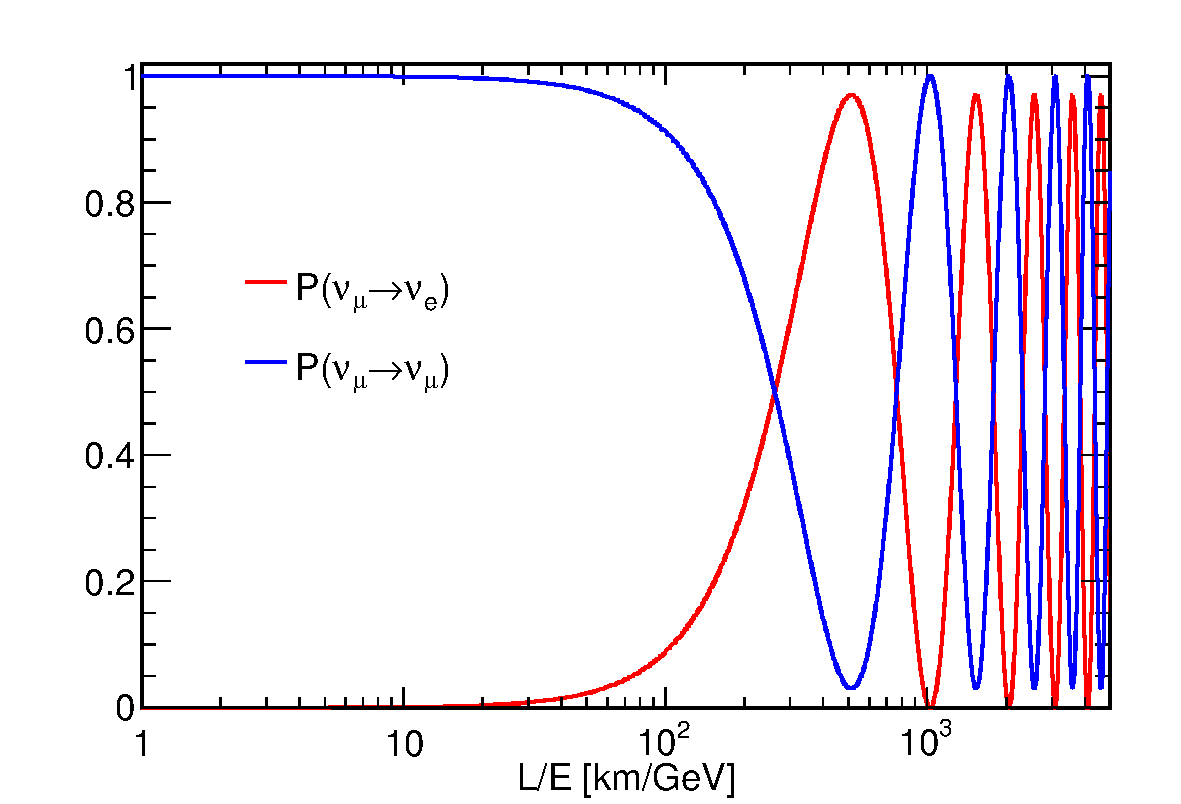
\includegraphics[width=.6\linewidth]{../figures/oscillation_prob.pdf}    
  \end{center}
  \begin{itemize}
\item Oscillation and survival probabilities for the two neutrino state with an initial $\nu_{\mu}$. The values for $\Delta m^2$ and $\sin^22\theta$ ($2.41\times 10^{-3}$ eV$^2$ and 0.97, respectively) are taken from 2013 MINOS result (PRL, 110, 251801)    
  \end{itemize}
\end{frame}

\begin{frame}
  \frametitle{See-Saw Model}
  \begin{itemize}
  \item Popular way to explain why there are light left-handed neutrinos and no observed right-handed neutrinos.
  \item Right-handed states would be sterile -- don't interact (or interact only very weakly) via weak weak interactions.
  \end{itemize}
  \begin{center}
    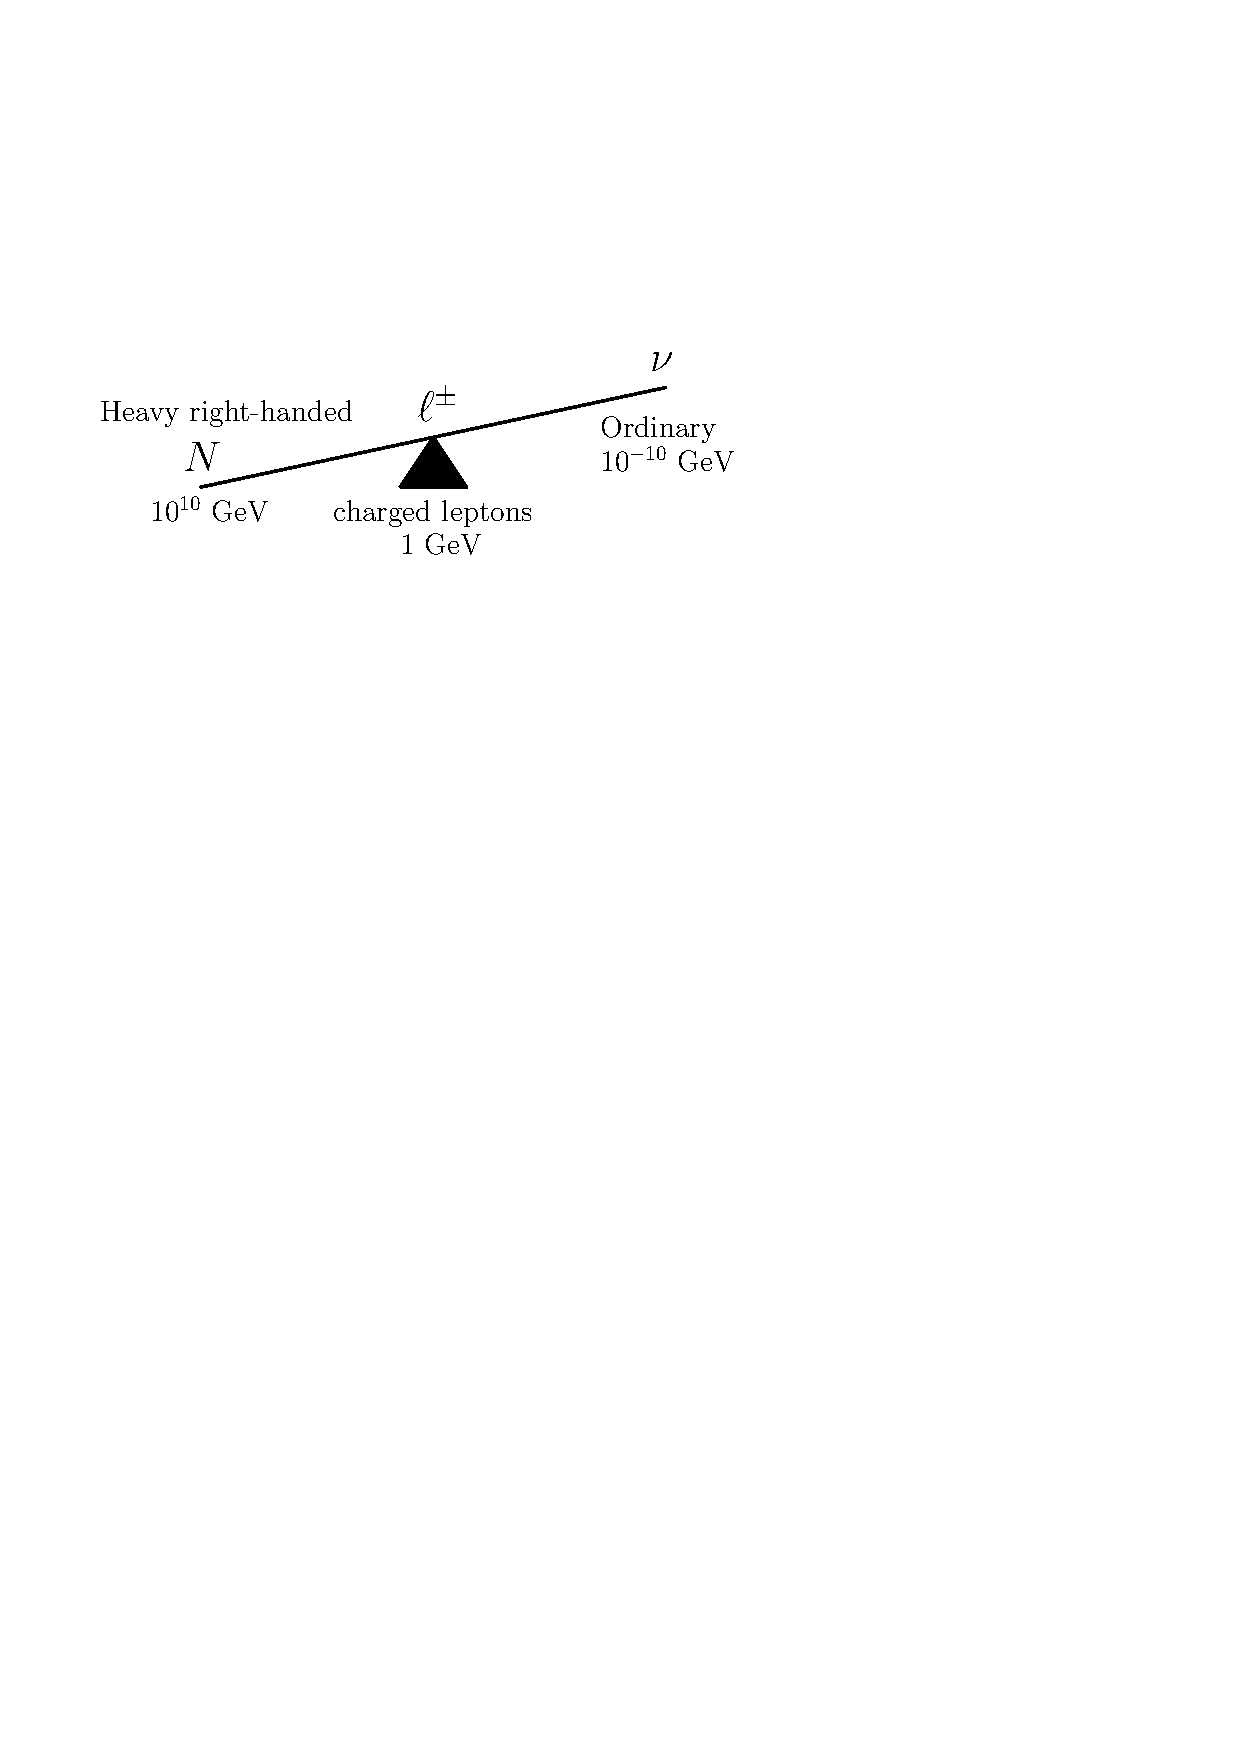
\includegraphics[width=.75\linewidth]{../figures/seesaw.pdf}
  \end{center}
\end{frame}

\begin{frame}
  \frametitle{See-Saw continued}
  \begin{align}
    \begin{split}
    \begin{pmatrix}
      \overline{\nu} & \overline{N}
    \end{pmatrix}
    \begin{pmatrix}
      0 & m_D \\
      m_D & M
    \end{pmatrix}
    \begin{pmatrix}
      \nu \\ N
    \end{pmatrix}
    \end{split}
  \end{align}
  \begin{itemize}
    \item For the Dirac mass much ness than $M$, eigenvalues are $-m_D^2/M$ and $M$, with eigenstates made from mostly $\nu$ and $N$, respectively.
    \item This means that as $M$ goes up or down $m_D^2/M$ does the opposite -- hence the See-Saw.
    \item We are left with light-left handed neutrinos and heavy right-handed.
    \item There are 3 types of See-Saw model (I, II, III) that involve the introduction of isospin singlets, scalar triplets, and fermion triplets.
    \item Drawing distinctions is beyond the scope of this project.
  \end{itemize}
\end{frame}

\begin{frame}
  \frametitle{The LSND Experiment}
  \footnotesize{
    \begin{columns}
      \begin{column}{.5\linewidth}      
        \begin{itemize}
        \item Liquid Scintillator Neutrino Detector.
        \item Los Alamos National Laboratory from 1993 to 1998.
        \item Cherenkov detector using 1220 PMTs.
        \item Protons strike target, use pions decaying at test to product $\overline{\nu}_\mu$.
        \end{itemize}
      \end{column}
      \begin{column}{.5\linewidth}
        \begin{itemize}
        \item $117.9 \pm 22.4$ events, signal excess of $87.9\pm 22.4 \pm 6.0$.
        \item $(\sin^2 2\theta,\Delta m^2)$ fit extracts allowed oscillation regions.
        \item Best fits yields $\Delta m^2 \sim 1$ eV.
        \item Disagrees with solar and atmospheric oscillation experiments and also LEP experiments for 3 light flavor neutrinos.
        \end{itemize}
      \end{column}
    \end{columns}
  }
  \begin{center}
    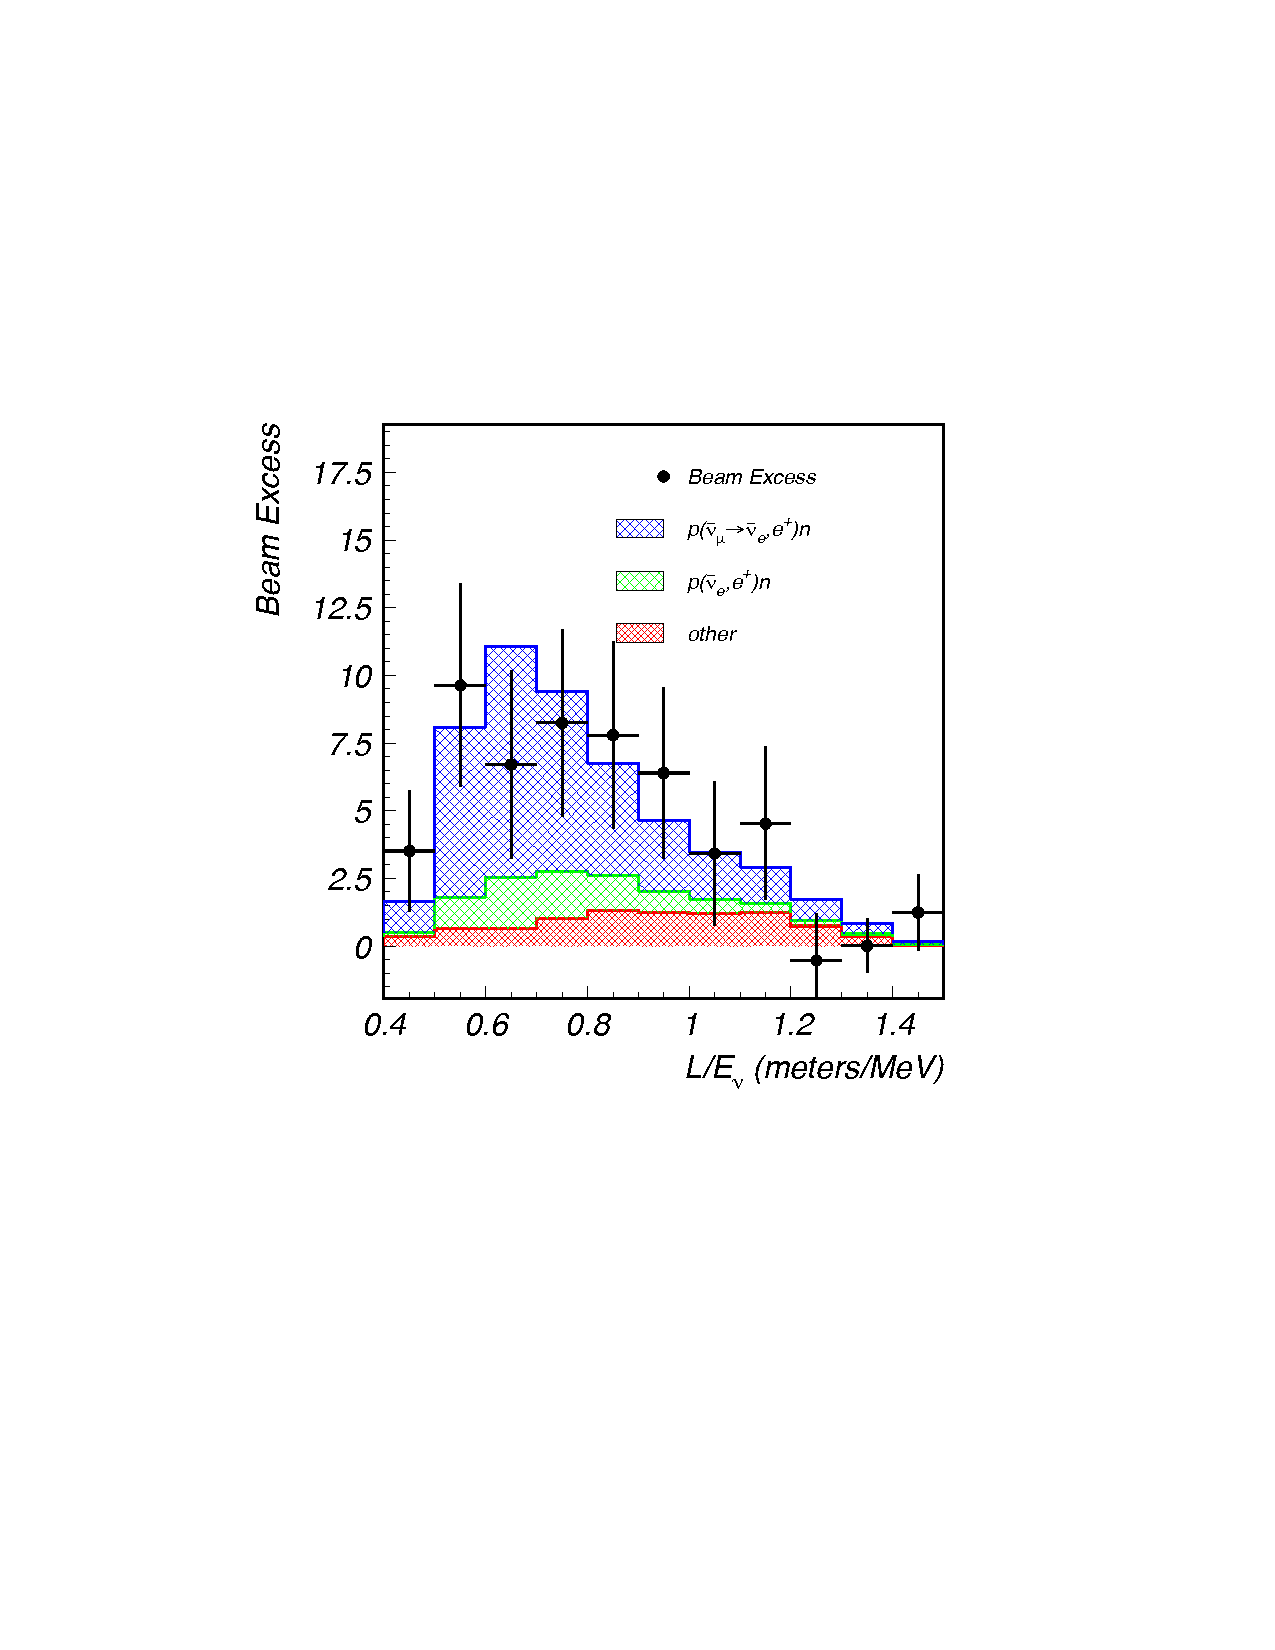
\includegraphics[width=.35\linewidth]{../figures/LSND_plot.pdf}
  \end{center}
\end{frame}
\begin{frame}
  \frametitle{The MiniBooNE Experiment}
  \scriptsize{
    \begin{columns}
      \begin{column}{.5\linewidth}      
        \begin{itemize}
        \item Developed to answer the LSND anomaly.
        \item Collected data at Fermilab from 2002 to 2012
        \item Cherenkov detector using PMTs (just like LSND)
        \item 8 GeV protons from the Booster strike beryllium target, pions decay producing neutrinos
          \begin{center}
            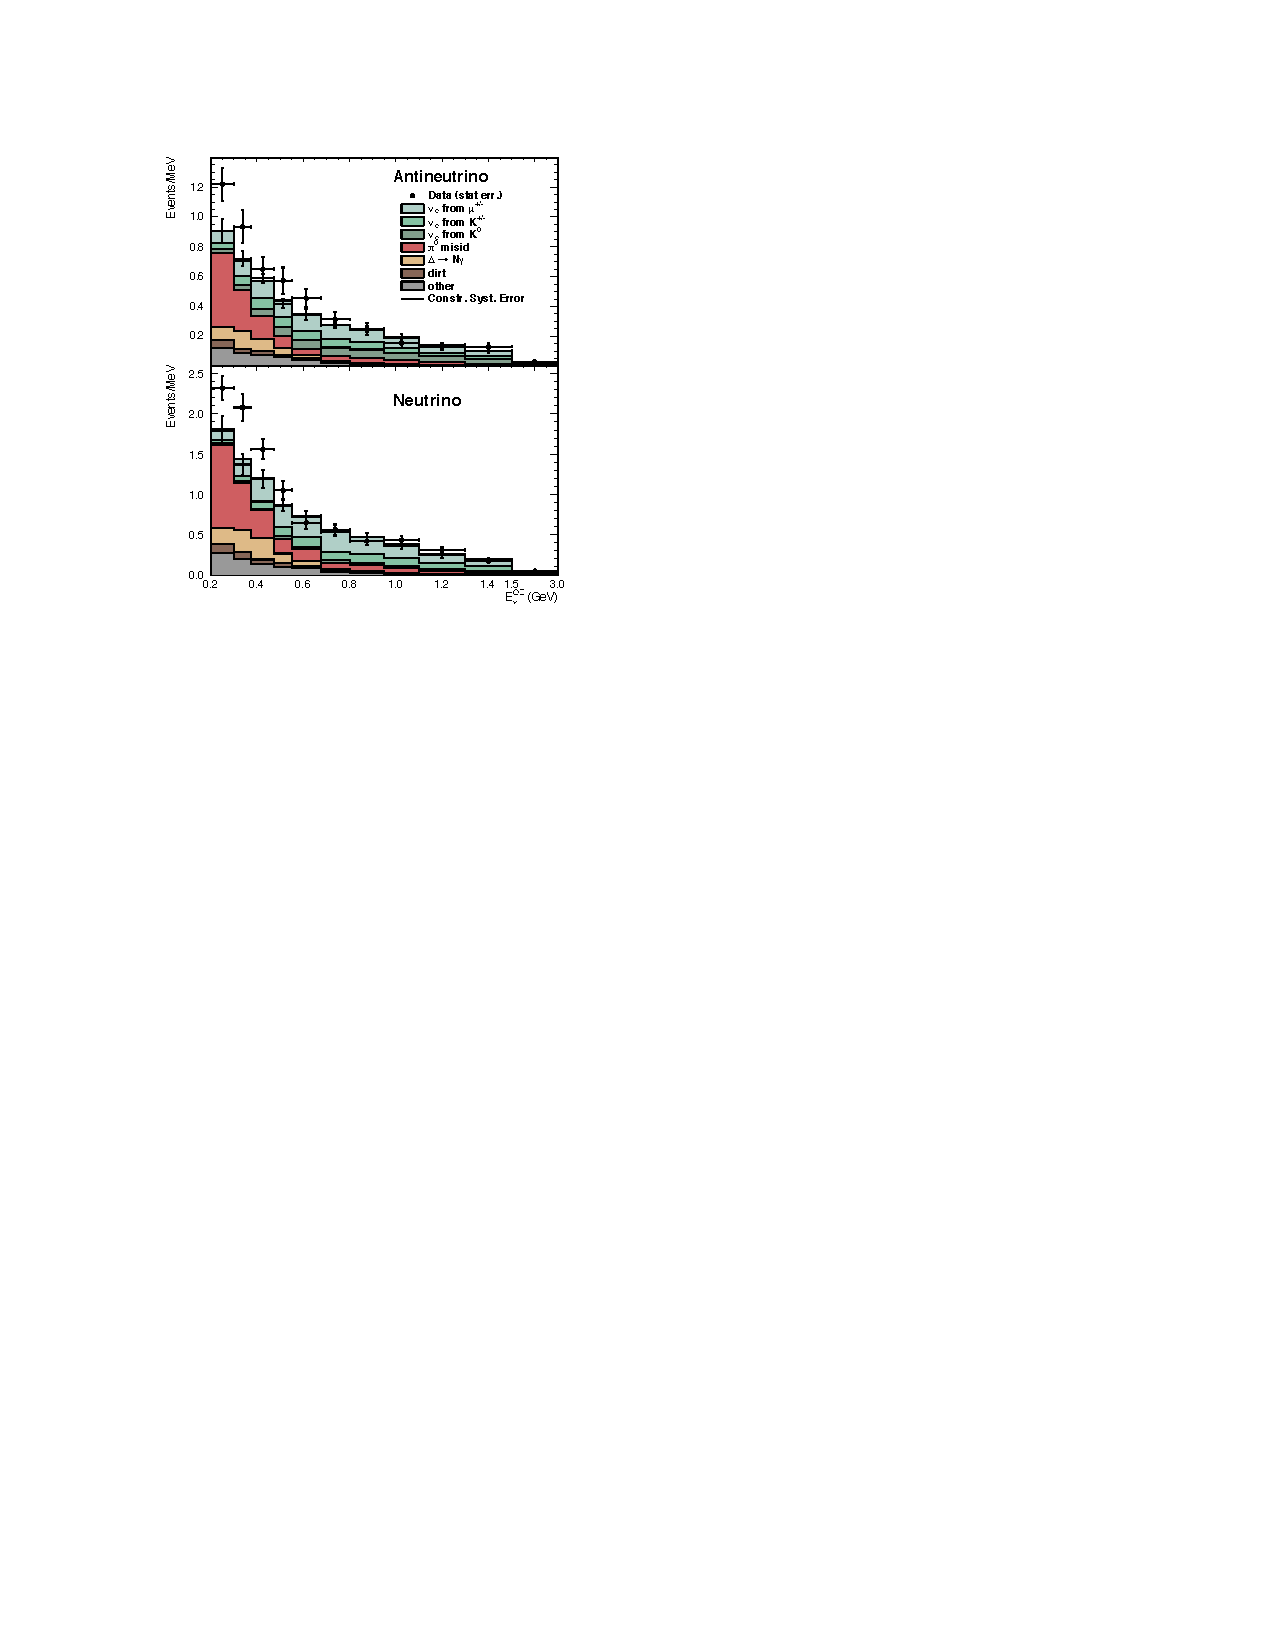
\includegraphics[width=.9\linewidth]{../figures/miniboone_excess.pdf}
          \end{center}
        \end{itemize}
      \end{column}
      \begin{column}{.5\linewidth}
        \begin{itemize}
        \item Consistent with the LSND anti neutrino oscillation result.
          \begin{center}
            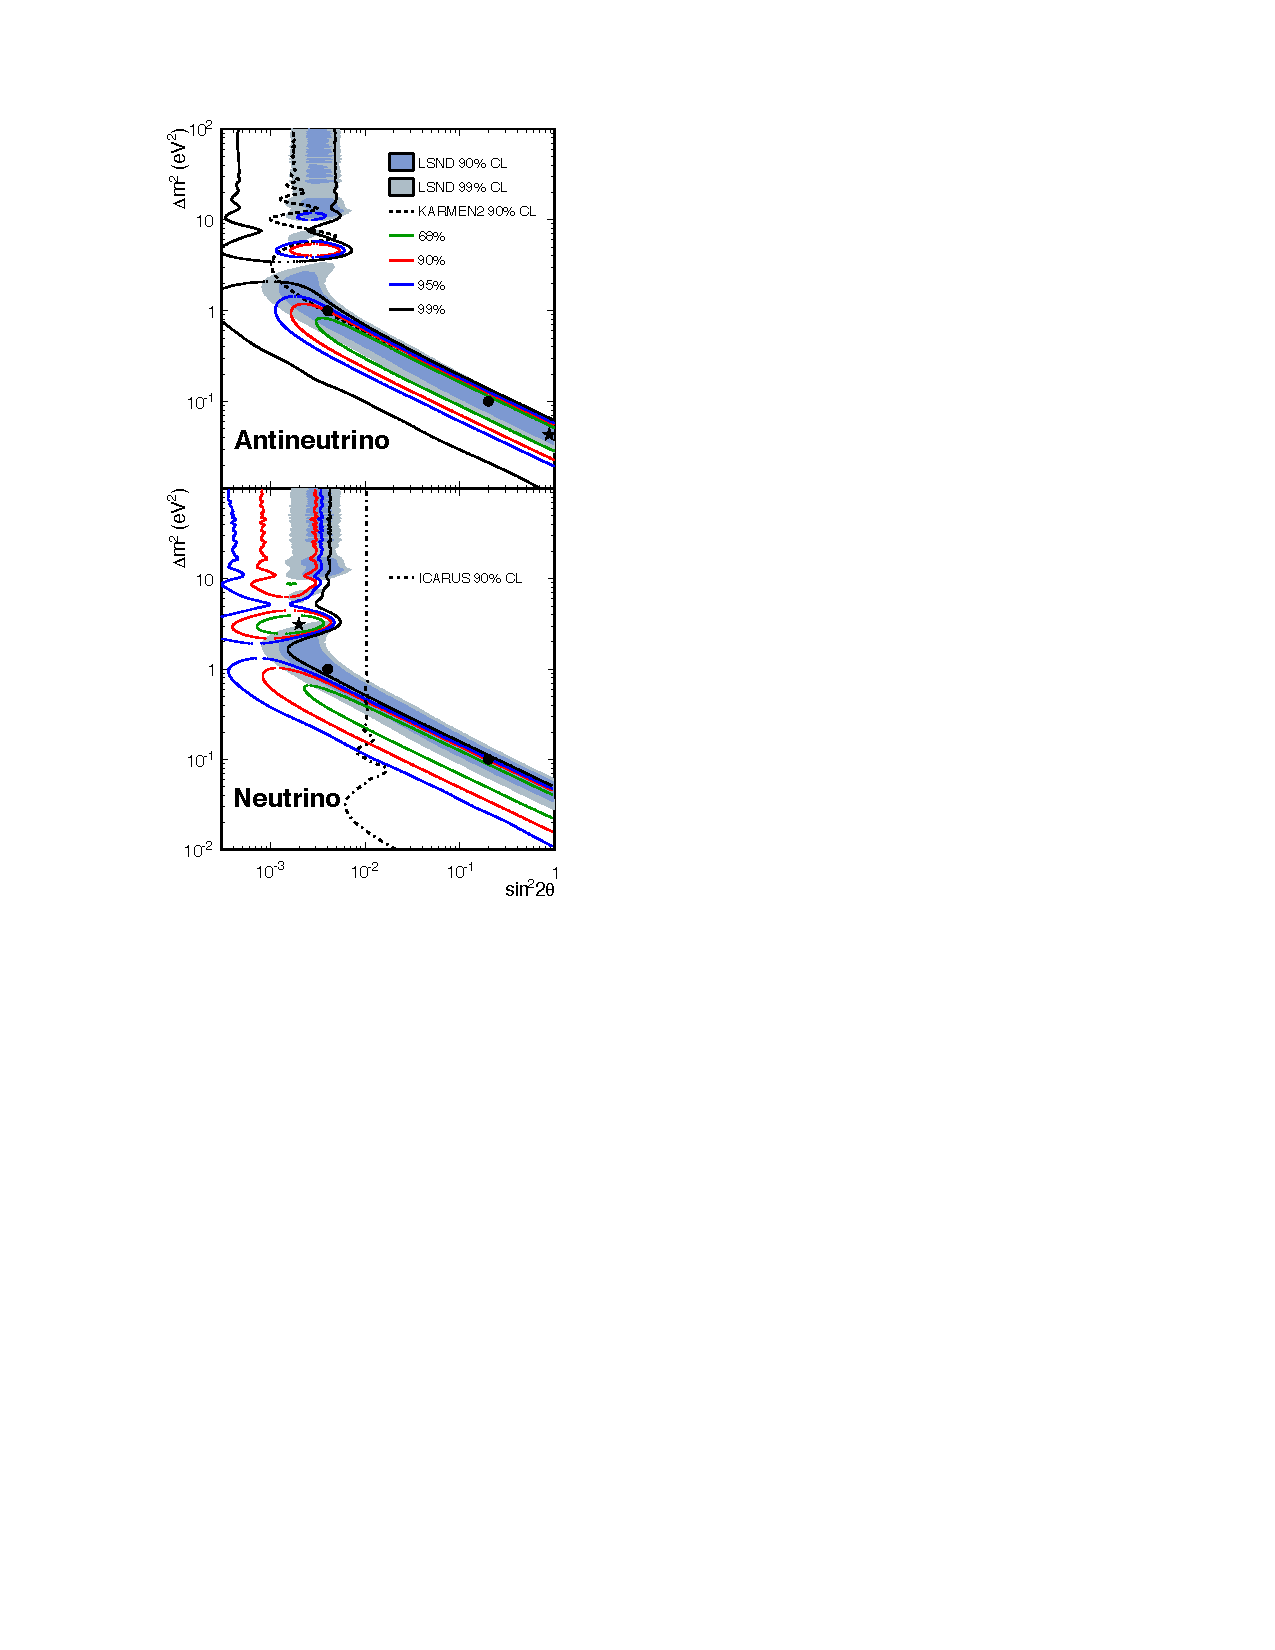
\includegraphics[width=.6\linewidth]{../figures/miniboone_regions.pdf}
          \end{center}
        \item Detector systematics make it difficult to differentiate between $\pi^0\rightarrow\gamma\gamma$ and an electron in the detector.
        \end{itemize}
      \end{column}
    \end{columns}
  }
\end{frame}




\begin{frame}
  \frametitle{The MINOS/MINOS+ Experiment}
  \begin{itemize}
  \item Long baseline, disappearance experiment
  \item Latest results now exclude much of the LSND allowed phase space
    \begin{center}
      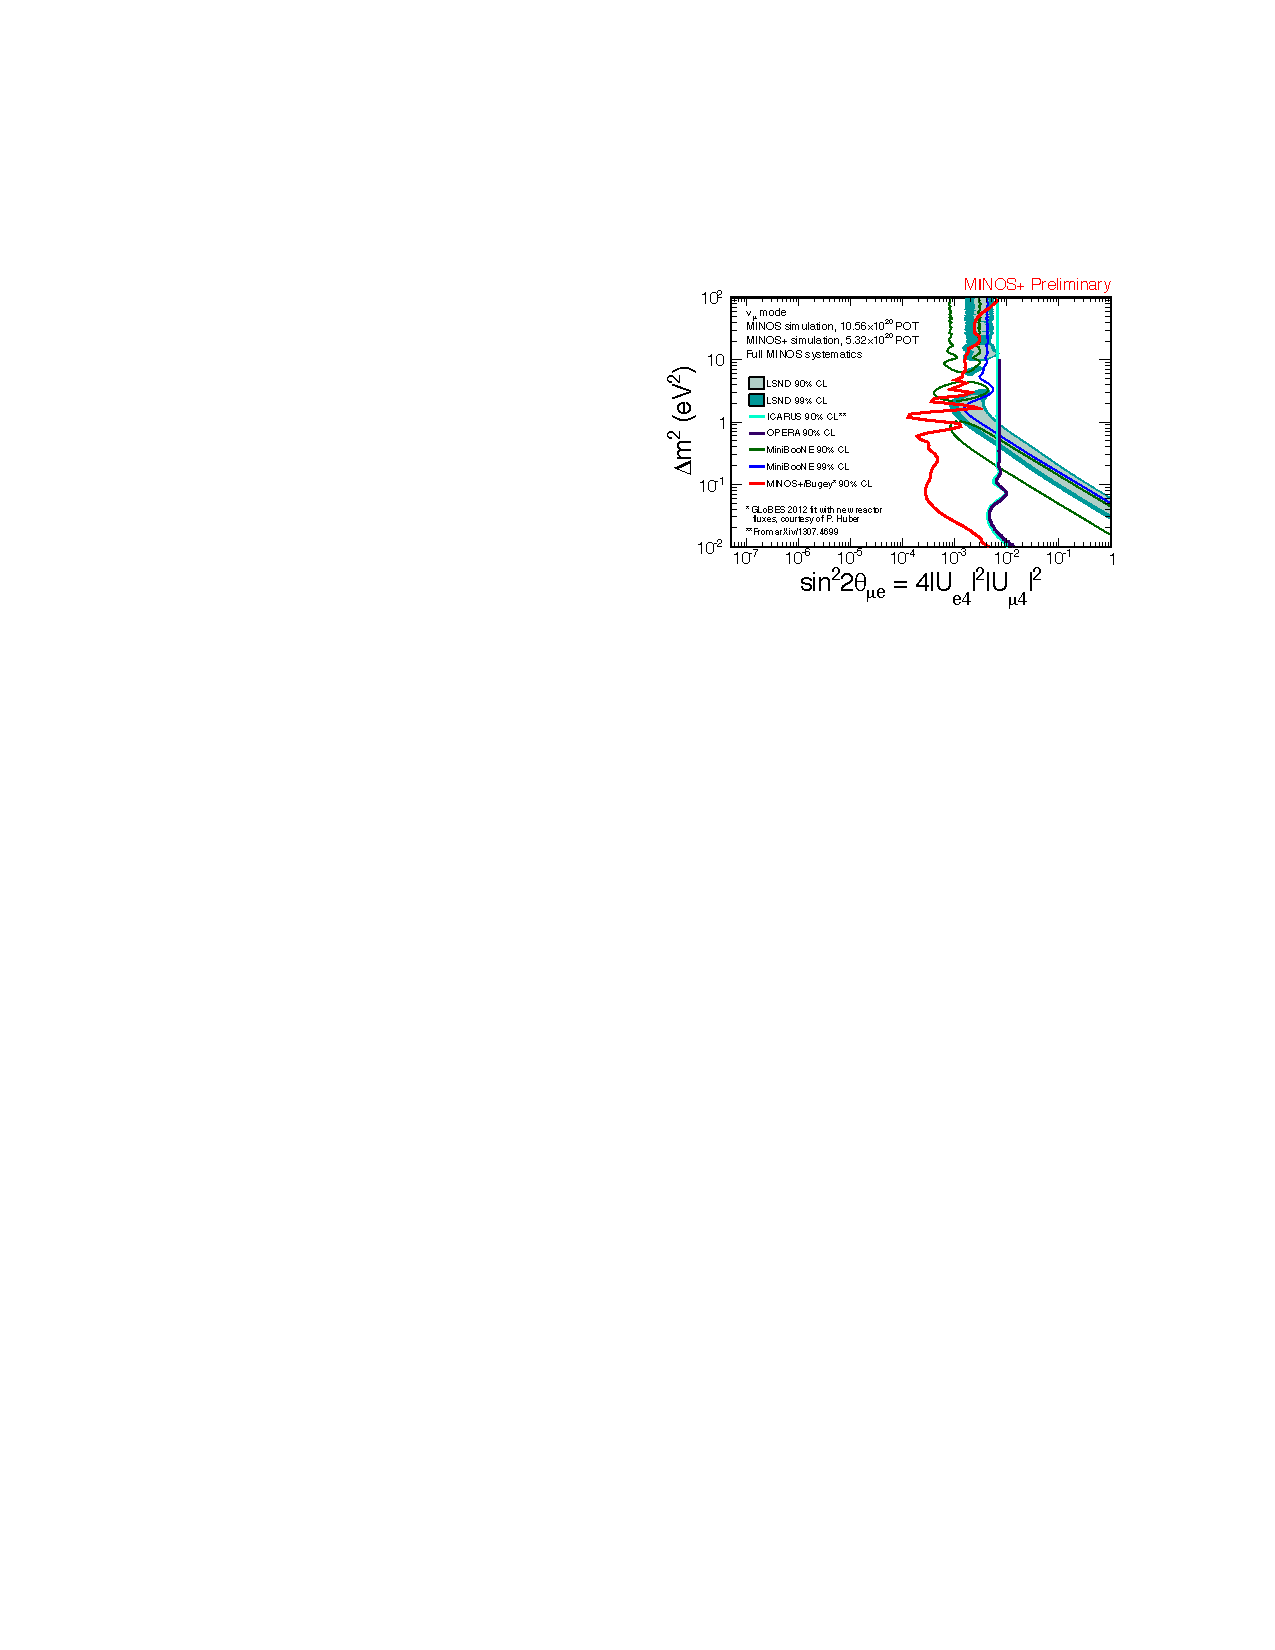
\includegraphics[width=.9\linewidth]{../figures/minos2.pdf}
    \end{center}
  \end{itemize}
\end{frame}

\begin{frame}
  \frametitle{The Super-Kamiokande Experiment}
  \begin{itemize}
  \item Atmospheric, TODO experiment
  \item Latest results TODO
    \begin{center}
      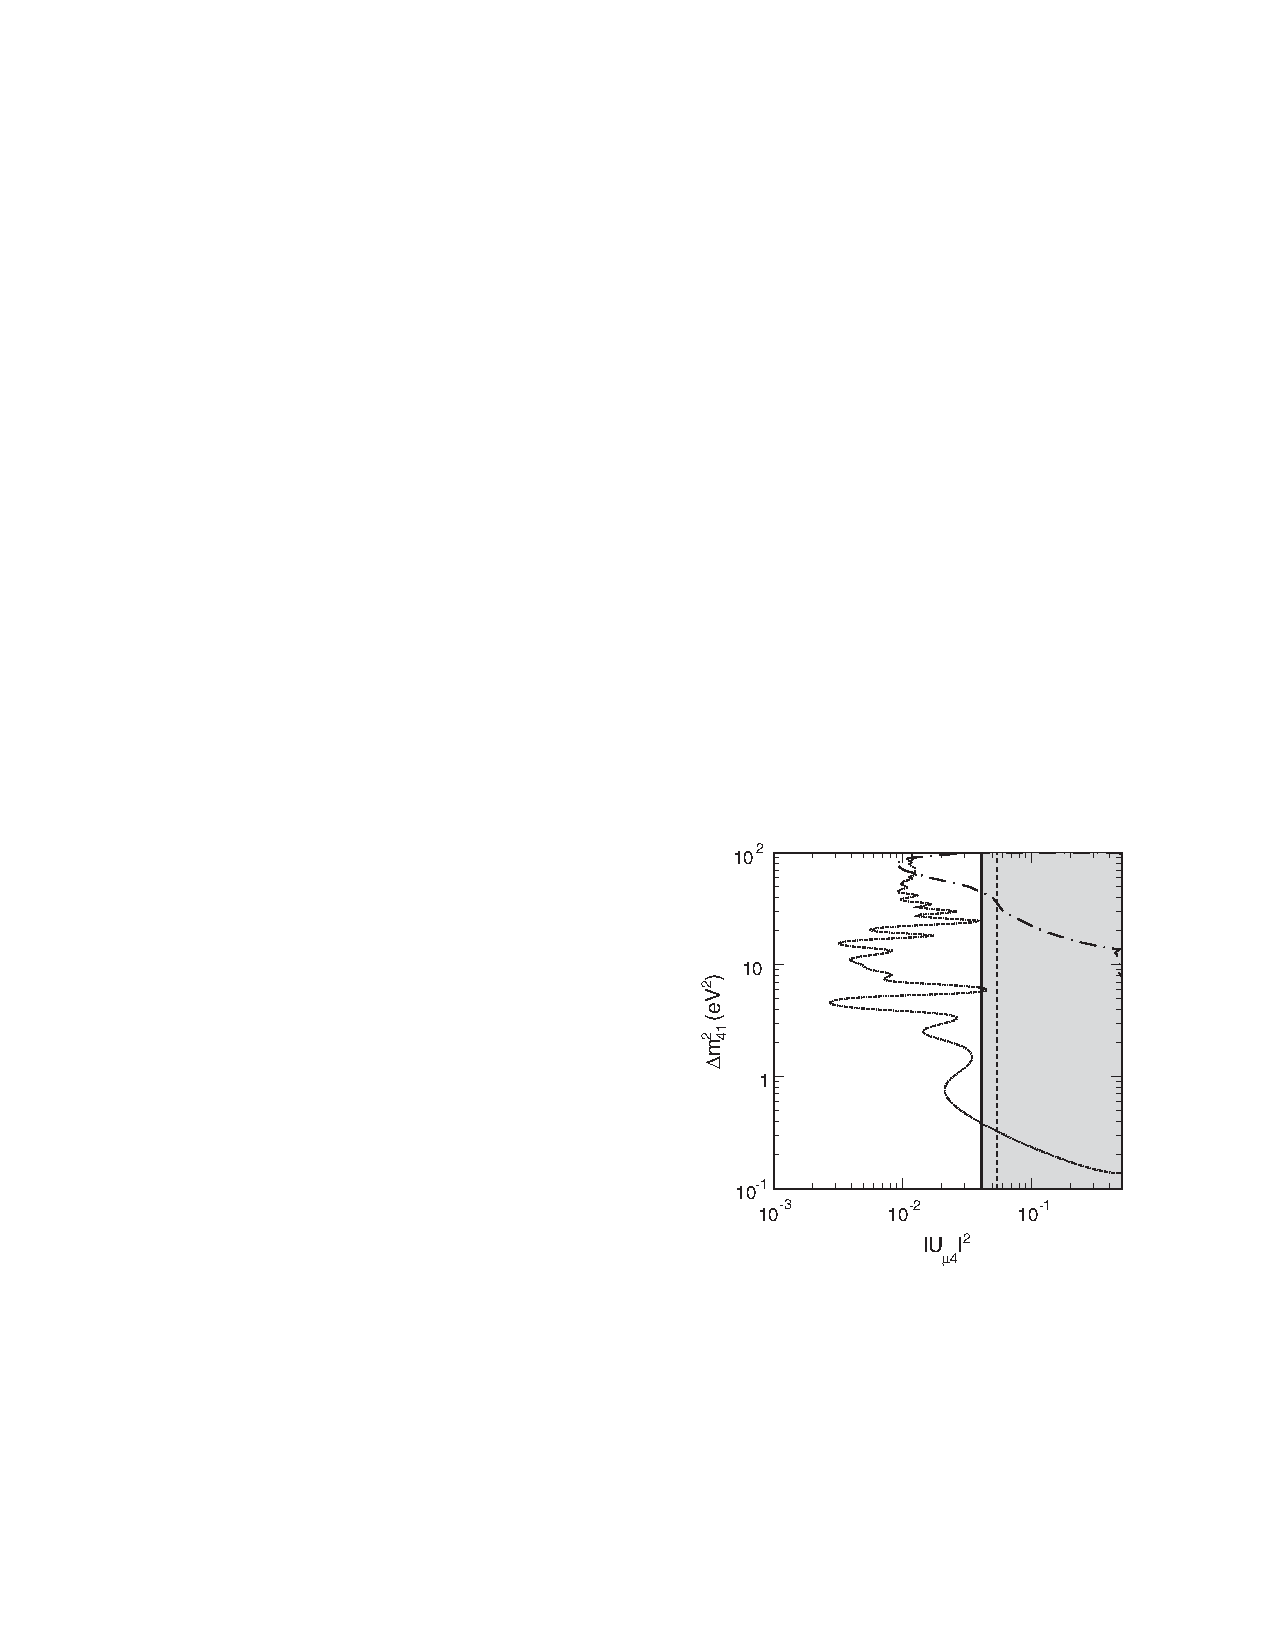
\includegraphics[width=.5\linewidth]{../figures/sk1.pdf}
    \end{center}
  \end{itemize}
\end{frame}

\begin{frame}
  \frametitle{The Daya Bay Experiment}
  \begin{itemize}
  \item Reactor, TODO experiment
  \item Latest results TODO
    \begin{center}
      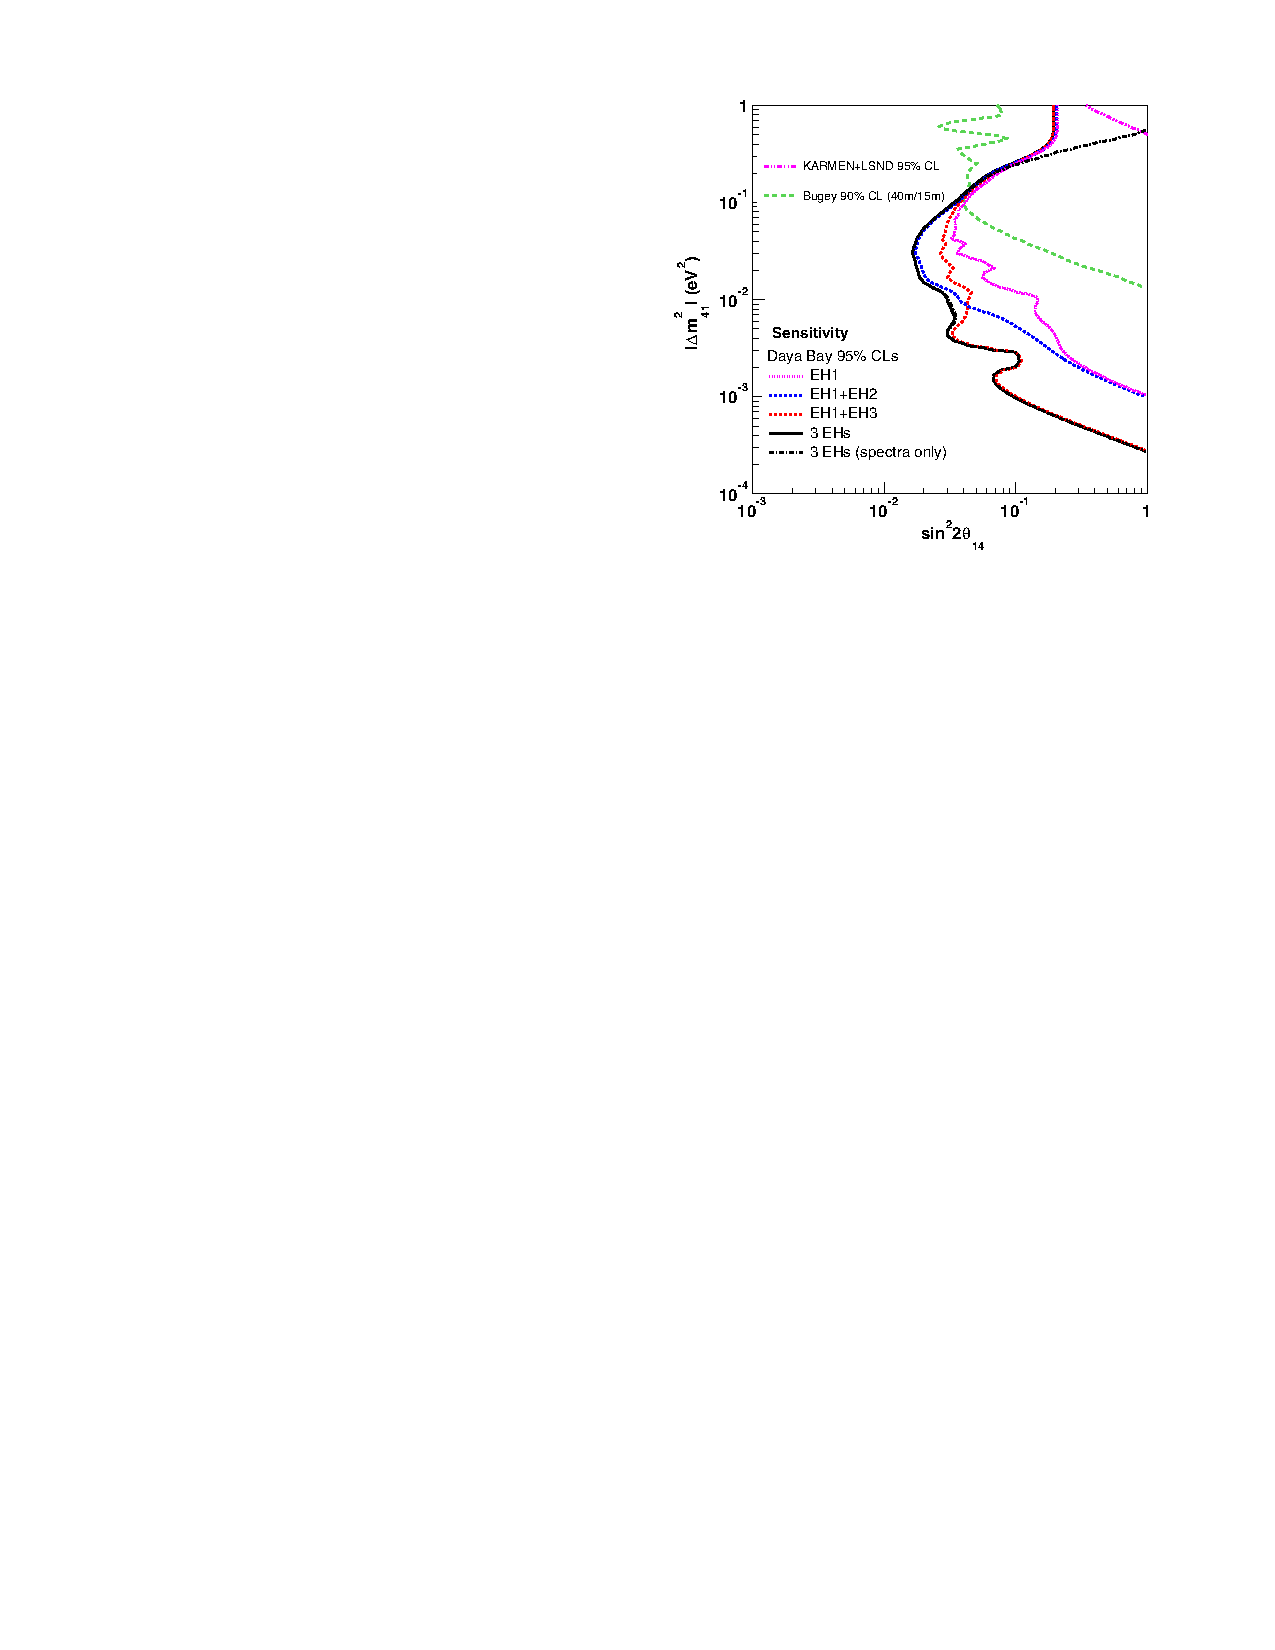
\includegraphics[width=.5\linewidth]{../figures/daya1.pdf}
    \end{center}
  \end{itemize}
\end{frame}


\begin{frame}
  \frametitle{Conclusions}
  \begin{itemize}
  \item Sterile neutrinos\ldots
  \end{itemize}
\end{frame}


\end{document}

%%%%%%%%%%%%%%%%%% 
%%%%%%%%%%%%%%%%%% 
%%%%%%%%%%%%%%%%%% 
%%%%%%%%%%%%%%%%%% 
%%%%%%%%%%%%%%%%%% 
%%%%%%%%%%%%%%%%%% 
%%%%%%%%%%%%%%%%%% 
%%%%%%%%%%%%%%%%%% 
%%%%%%%%%%%%%%%%%% 
%%%%%%%%%%%%%%%%%% 
%%%%%%%%%%%%%%%%%% 
%%%%%%%%%%%%%%%%%% 
%%%%%%%%%%%%%%%%%% 
%%%%%%%%%%%%%%%%%% 
%%%%%%%%%%%%%%%%%% 
%%%%%%%%%%%%%%%%%% 
%%%%%%%%%%%%%%%%%% 
%%%%%%%%%%%%%%%%%% 
%%%%%%%%%%%%%%%%%% 
%%%%%%%%%%%%%%%%%% 
%%%%%%%%%%%%%%%%%% 
%%%%%%%%%%%%%%%%%% 
%%%%%%%%%%%%%%%%%% 
%%%%%%%%%%%%%%%%%% 
%%%%%%%%%%%%%%%%%% 
%%%%%%%%%%%%%%%%%% 
%%%%%%%%%%%%%%%%%% 
%%%%%%%%%%%%%%%%%% 
%%%%%%%%%%%%%%%%%% 
%%%%%%%%%%%%%%%%%% 
%%%%%%%%%%%%%%%%%% 
%%%%%%%%%%%%%%%%%% 

% \DeclareRobustCommand{\su3flavor}{$\text{SU(3)}_{\text{flavor}}$}
% \DeclareRobustCommand{\qqbar}{$q\overline{q}$}


\begin{frame}
  \frametitle{Introduction}
  \begin{itemize}
  \item Mesons are defined as particle resonances with baryon number 0.
    \begin{align}
      B_n = \frac{1}{3}\left(n_q-n_{\overline{q}}\right) = 0
    \end{align}
  \item Therefore, mesons can be defined as any bound state containing and equal number of quarks and antiquarks (or none of each).
  \item We will discuss three types of mesons beyond \su3flavor \qqbar: QCD Hybrids, Glueballs, and Tetraquarks.
  \end{itemize}
\end{frame}

\begin{frame}
  \frametitle{QCD Hybrids}
  \begin{itemize}
  \item `Normal'  mesons are color--anticolor \su3flavor \qqbar~states.
    \begin{itemize}
    \item Gluon field binding the quarks implicitly assumed to be colorless, with vacuum quantum numbers.
    \end{itemize}
  \item Calculating \qqbar~meson quantum numbers:
    \begin{itemize}
    \item $S = 0, 1$; $L = 0, 1, 2, \ldots$; $J = L+S, L+S-1, \ldots, \left| L-S \right|$
    \item $P = (-1)^{L+1},~C = (-1)^{L+S}$
    \end{itemize}
  \item Allowed $J^{PC} = 0^{-+}, 0^{++}, 1^{--}, 1^{+-}, 1^{++}, 2^{--}, 2^{-+}, 2^{++},\ldots$ for (neutral) \su3flavor \qqbar~mesons \cite{ketzer}.
  \item Other $J^{PC}$'s such as $J^{PC} = 0^{--}, 0^{+-}, 1^{-+}, 2^{+-},\ldots$ are considered `exotic'.
  \end{itemize}
\end{frame}

\begin{frame}
  \frametitle{QCD Hybrids -- Continued}
  \begin{itemize}
  \item Full QCD approach allows for a wider variety of mesons:
    \begin{itemize}
    \item Gluon field can have a net color, opposite to the quark's net color.
    \item Gluon field can also take different quantum numbers.
    \end{itemize}
  \item Such mesons are called QCD hybrid's.
    \begin{itemize}
    \item Includes mesons with more than one \qqbar~pair.
    \end{itemize}
  \item Hybrids with allowed \su3flavor quantum numbers are difficult to detect experimentally; appear as an excess.
  \item Hybrids with exotic $J^{PC}$ quantum numbers easy to detect experimentally; ``smoking gun''.
  \end{itemize}
\end{frame}

\begin{frame}
  \frametitle{QCD Hybrids -- Continued}
  \begin{itemize}
  \item Non-perturbative/lattice QCD needed to calculate QCD hybrid's properties.
  \item Lattice QCD can work from first principles, but the results have large uncertainties and can depend on the specific methods used.
  \item Experimental measurements of QCD hybrids would help clarify the theoretical picture.
  \end{itemize}
\end{frame}

\begin{frame}
  \frametitle{Glueballs}
  \begin{itemize}
  \item Gluons carry color charge and interact through the strong force.
  \item A glueball can be two or three (or more) gluons bound to one another in the absence of quarks.  It is color neutral.
    \begin{align}
      |gg\rangle, |ggg\rangle, |ggg\ldots\rangle
    \end{align}
  \item There are no experimentally confirmed glueballs – though there are several candidates.
  \end{itemize}
\end{frame}

\begin{frame}
  \frametitle{Glueballs -- Continued}
  \begin{itemize}
  \item They exhibit significant mixing with mesons
  \item The masses of the lighest glueballs are predicted to be around the same mass as known standard mesons
  \item QCD sum rule is a popular technique for calculating glueball masses
  \end{itemize}
  \begin{center}
    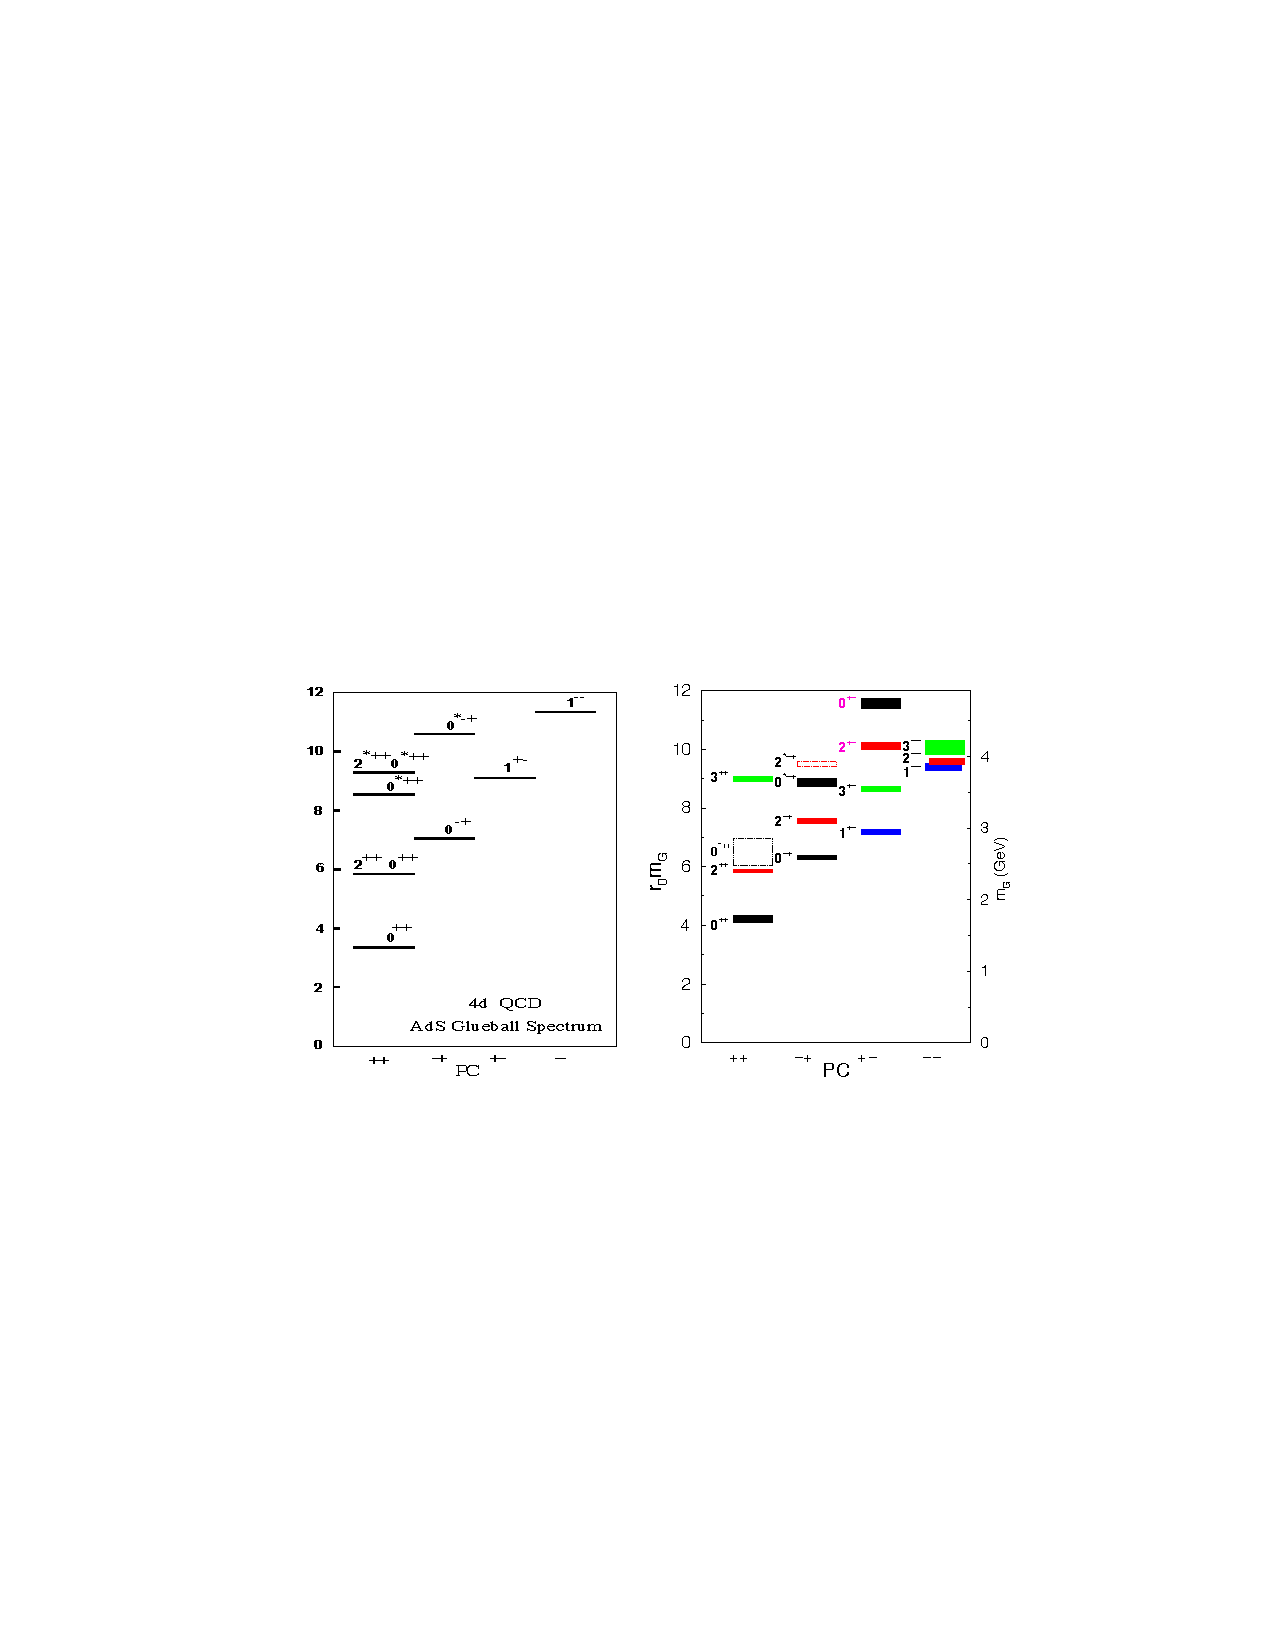
\includegraphics[width=.725\linewidth]{../figures/glueballmass.pdf}
  \end{center}
\end{frame}

\begin{frame}
  \frametitle{Tetraquarks}
  \begin{itemize}
  \item A 4 quark meson of the $|qq\overline{q}\overline{q}\rangle$ variety.
  \item Not two standard mesons interacting with one another (though this is how it might decay).
  \item Experimentally confirmed with $Z(4430)$.
  \item Higher numbers of quark groups have been theorized (pentaquarks, and more).
  \item Allowed by Lattice QCD.
  \end{itemize}
  \begin{center}
    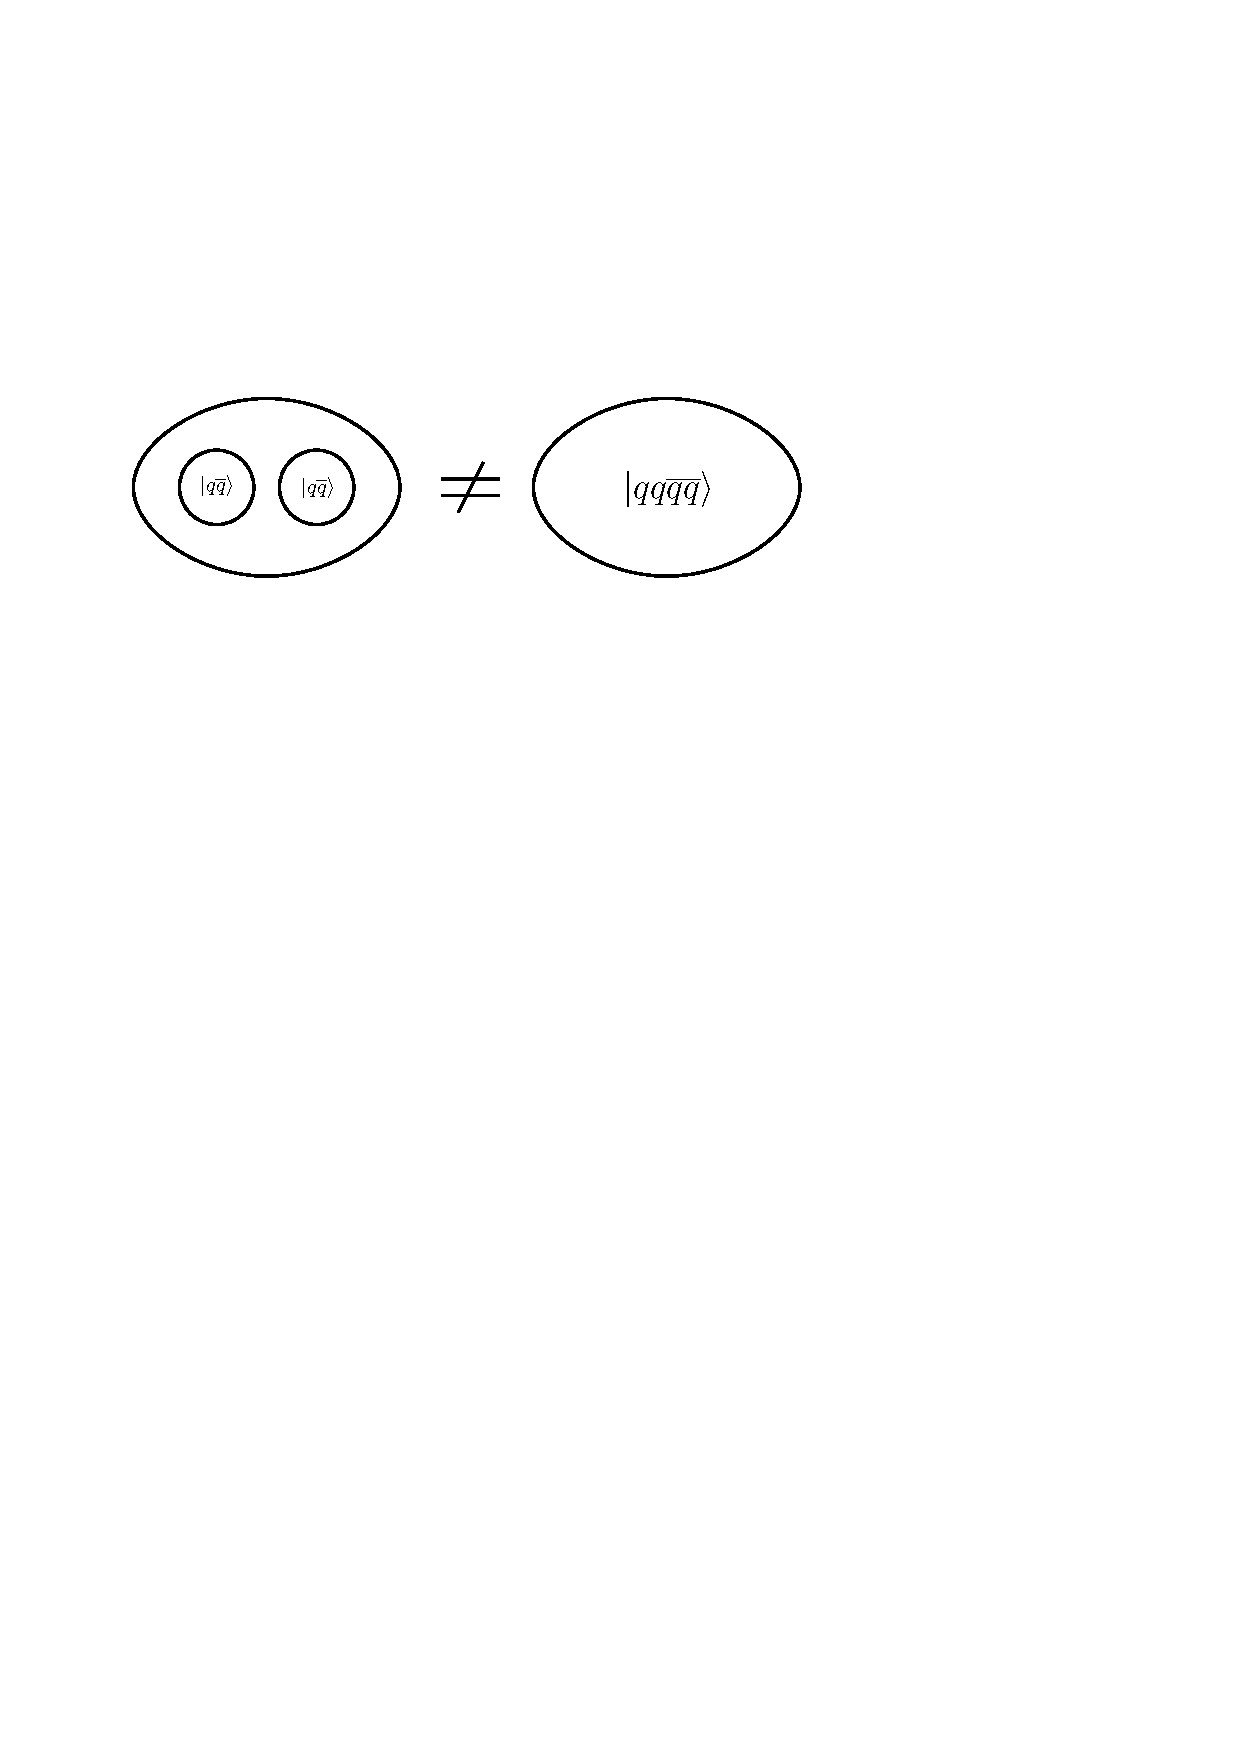
\includegraphics[width=.7\linewidth]{../figures/tetra.pdf}
  \end{center}
\end{frame}

\begin{frame}
  \frametitle{$\pi_1(1400)$ and $\pi_1(1600)$ -- Theoretical Prediction \& The Peripheral Experiments}
  \begin{itemize}
  \item Both the QCD String (QCD flux tube) Model and the Latice QCD model predict the hybrid exotic meson with $J^{PC}=1^{-+}$ around $1.9\pm 0.2$ GeV.
  \item Bag model predicts the exotic $J^{PC} = 1^{-+}$ at lower mass about $1.4$ GeV.
  \item Hybrid Mesons are expected to decay mainly into pairs of S- and P-wave mesons
  \item $\pi_1(1400)$, reported in the reaction $\pi^− p \rightarrow \eta \pi^− p$ at 18.3 GeV/$c$ by the E852 collaboration using the multi-particle Spectrometer (MPS) at the AGS.
  \item $\pi_1(1600)$, reported in the reaction $\pi^- p \rightarrow \pi^- \pi^- \pi^+ p$ at 18.3 GeV/$c$ by the E852
  \end{itemize}
\end{frame}

\begin{frame}
  \frametitle{$\pi_1(1400)$ Peripheral Experimental Results}
  \begin{center}
    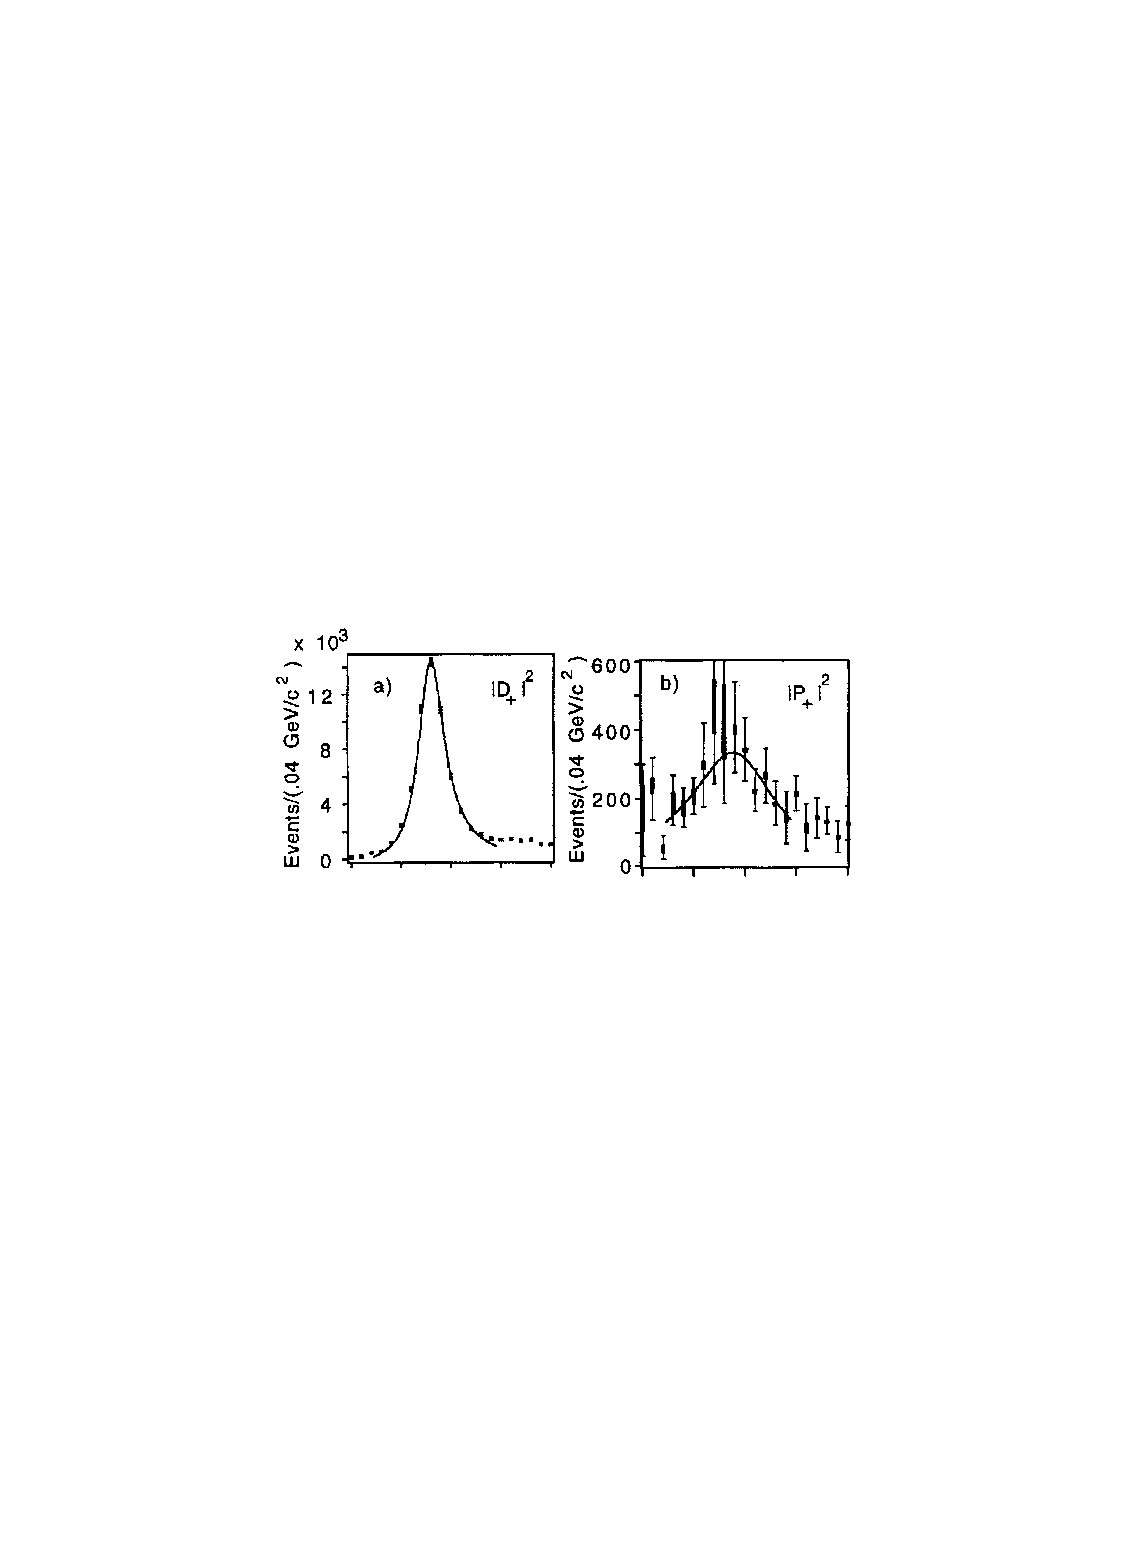
\includegraphics[width=.75\linewidth]{../figures/ping35.pdf}
  \end{center}
  \small{
    \begin{itemize}
    \item (L) Neutral parity exchange intensity. (R) Exotic parity exchange intensity.
    \item The peak in the $D_+$ amplitude is due to the $a_2(1320)$ meson, the peak in the $P_+$ amplitude is due to the exotic $\pi_1(1400)$. The exotic intensity is a small fraction (about 3\%) of the dominating $a_2(1320)$ contribution.
    \item Interation: $\pi^- p \rightarrow \eta\pi^-p$ (Intensity for the $\eta\pi^-$ system).
    \end{itemize}}
\end{frame}


\begin{frame}
  \frametitle{$\pi_1(1600)$ Peripheral Experimental Results}
  \begin{center}
    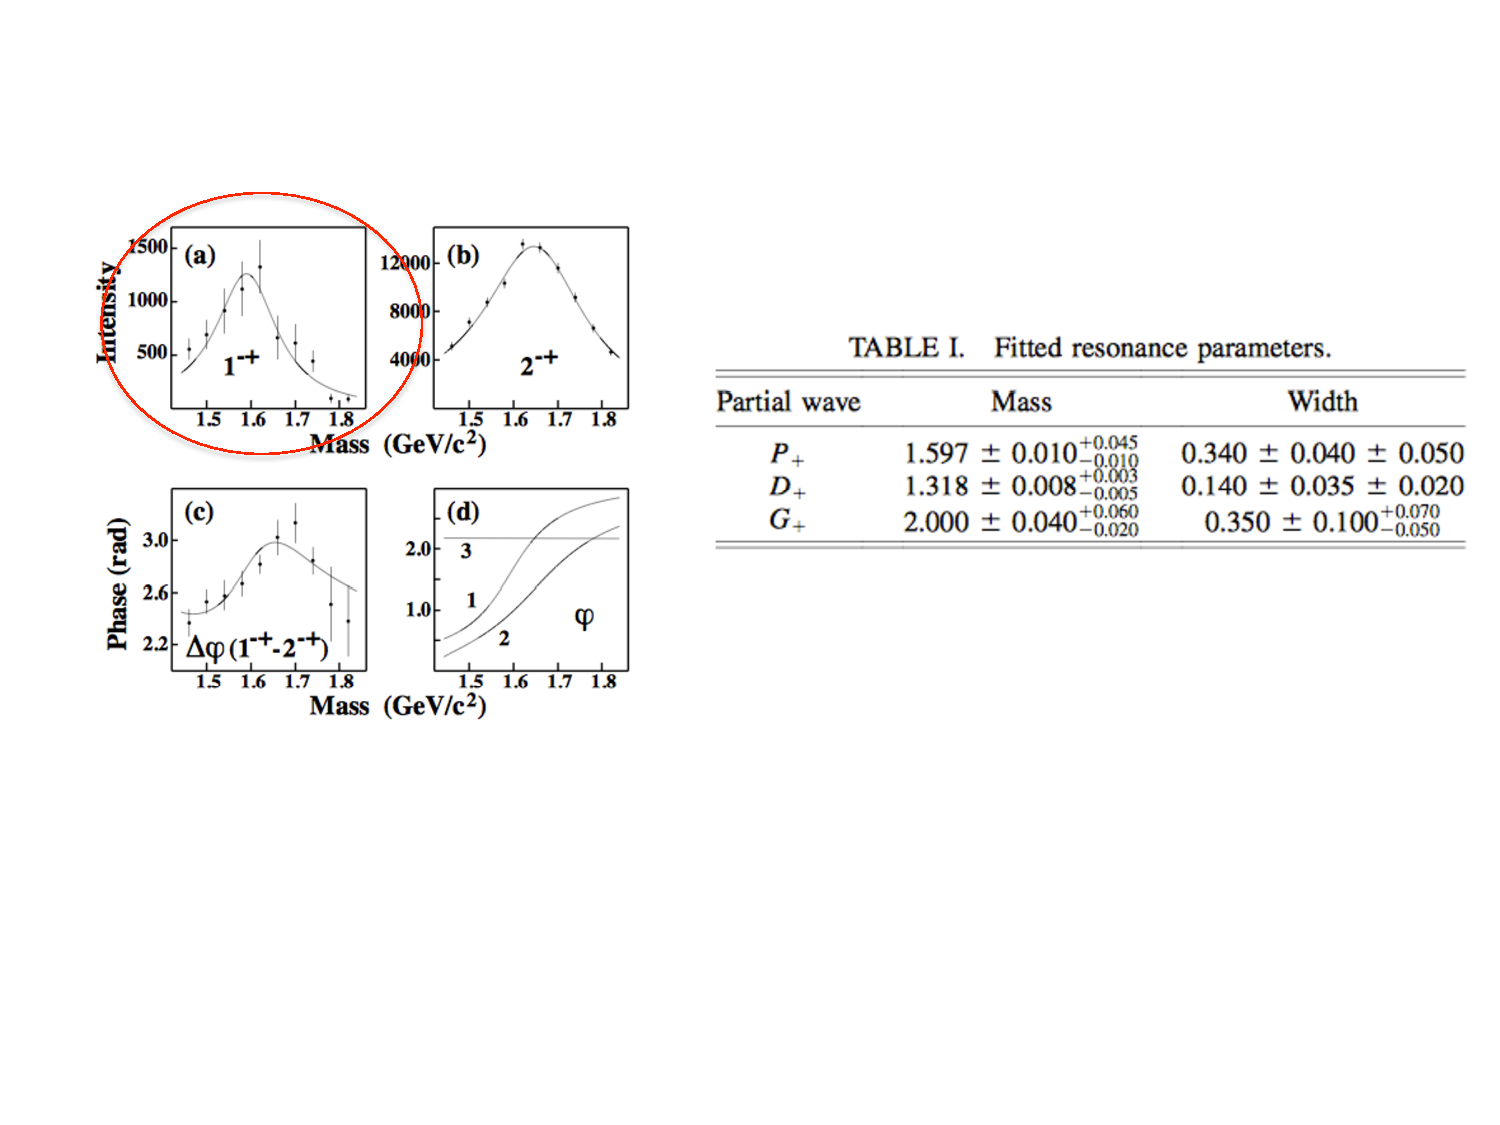
\includegraphics[width=.95\linewidth]{../figures/ping1600.pdf}
  \end{center}
  \small{
    \begin{itemize}
    \item $\pi_1(1600)$ decays into two pseudoscalar mesons. $\pi^- p\rightarrow \eta^{\prime} \pi^- p$. $\eta^{\prime}$ decays into $\eta$ and is reconstructed by $\eta\rightarrow\gamma\gamma$ The properties are consistent with the previous found exotic resonance $\pi_1(1600)$ from decay $\pi^- p \rightarrow \pi^- \pi^- \pi^+ p$.
    \end{itemize}}
\end{frame}

\begin{frame}
  \frametitle{$\pi_1(1400)$ and $\pi_1(1600)$ Peripheral and Annihilation Conclusions}
  \begin{center}
    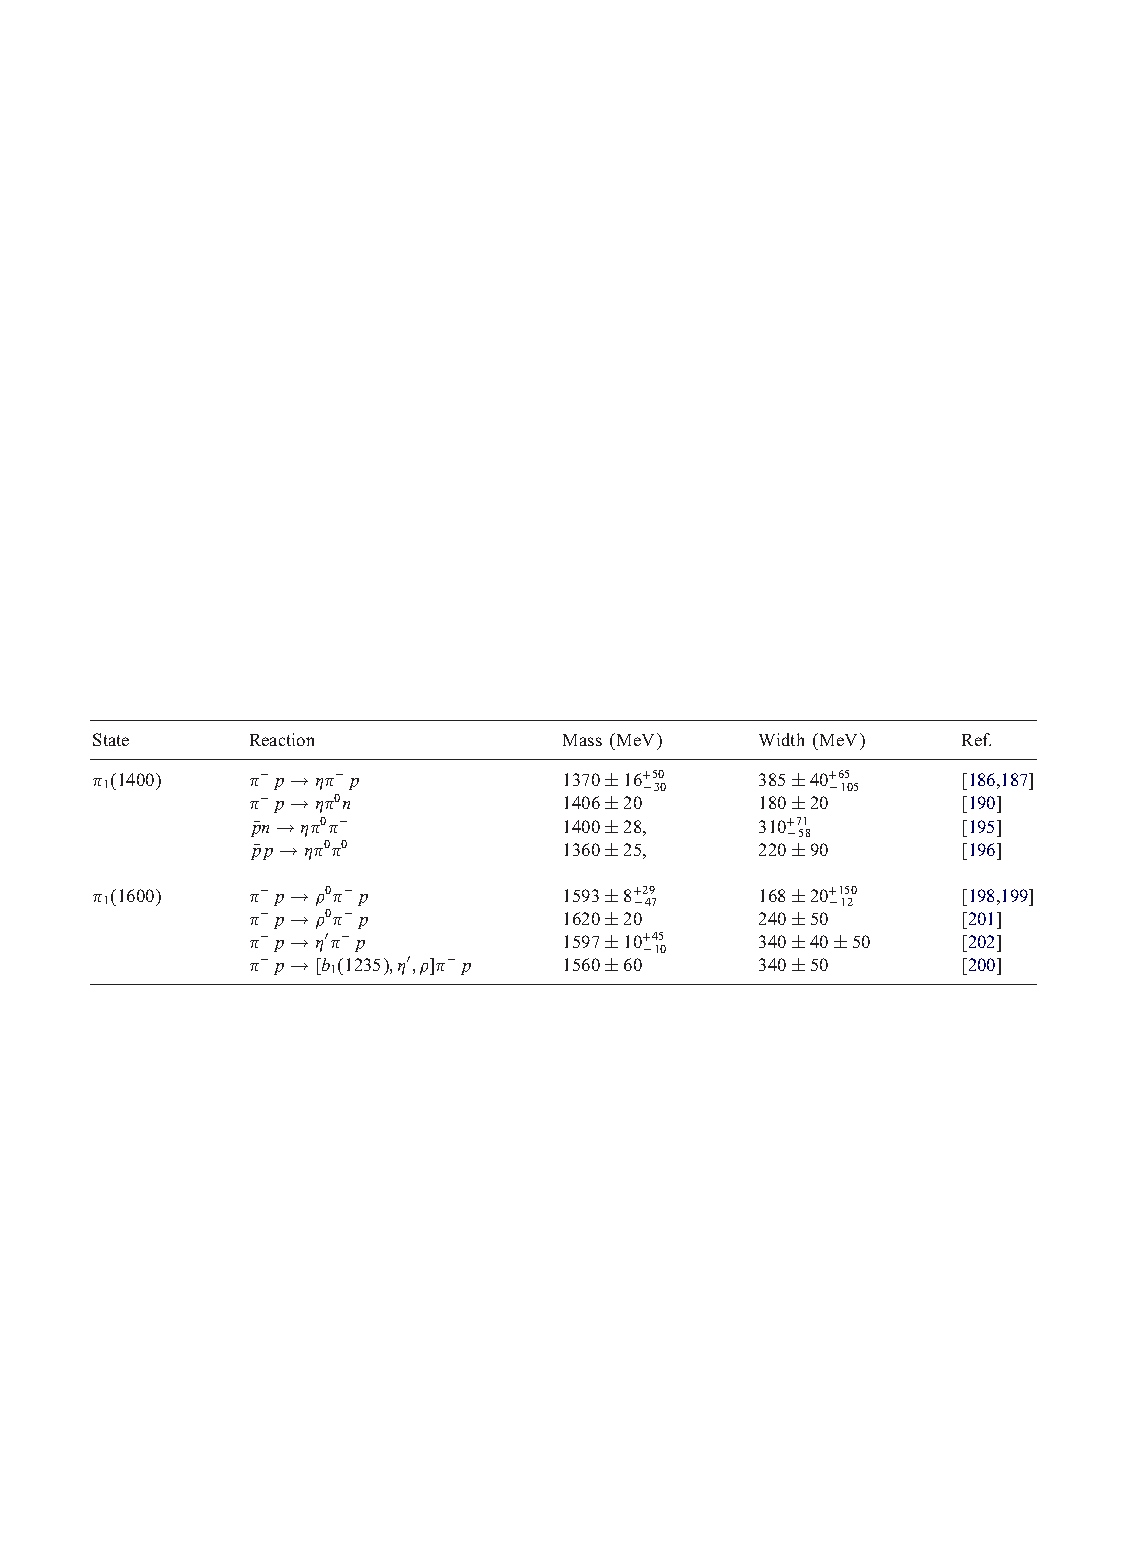
\includegraphics[width=.9\linewidth]{../figures/pingtable.pdf}
  \end{center}
  \begin{itemize}
  \item There are also $p\overline{p}$ annihilation experiments evidence for $\pi_1(1400)$ as isovectors, not glueballs. Decays also in favor of hybrids.
    Mass is below theory predictions. Future examinations are ongoing.
  \end{itemize}
\end{frame}

\begin{frame}
  \frametitle{The $Z(4430)$ at $B$ Factories}
  \small{
    \begin{itemize}
    \item Evidence of a charged tetraquark candidate at approximately 4430 MeV was observed by the Belle Collaboration in 2007. BaBar could not confirm.
    \item Charged state ruled out simply excited charmonium state.
    \item Resonant structures from $B^0 \rightarrow \psi^{\prime}\pi K$ decay.
    \item $J^P$ was unknown at the time and other models were possible (not a definite non-$q\overline{q}$ meson). The mass is very close to mass of $D^+_1\overline{D}^{*0} + D^{*+}\overline{D}_1^0$. Suspected to possibly be a $D$ ``molecule.''
    \end{itemize}
    \begin{center}
      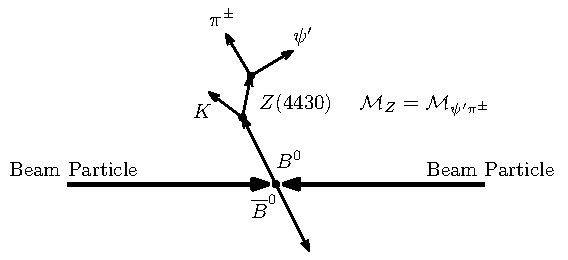
\includegraphics[width=.8\linewidth]{../figures/Z4430_diagram.pdf}
    \end{center}
  }
\end{frame}

\begin{frame}
  \frametitle{The $Z(4430)$ at the LHC}
  \small{
    \begin{itemize}
    \item In 2014 LHCb experiment confirmed the resonance at 13.9$\sigma$ and also confirmed $J^P$ of $1^+$, supporting the tetraquark candidate over the $D$ ``molecule'' candidate.
    \item Minimum quark content of $c\overline{c}d\overline{u}$.
    \item $m_{Z^{-}} = 4475 \pm 7^{+15}_{-25}$ MeV. $\Gamma_{Z^{-}} = 172 \pm 13^{+37}_{-34}$ MeV.
    \end{itemize}
    \begin{center}
      \begin{columns}
        \begin{column}{.5\linewidth}
          \begin{center}
            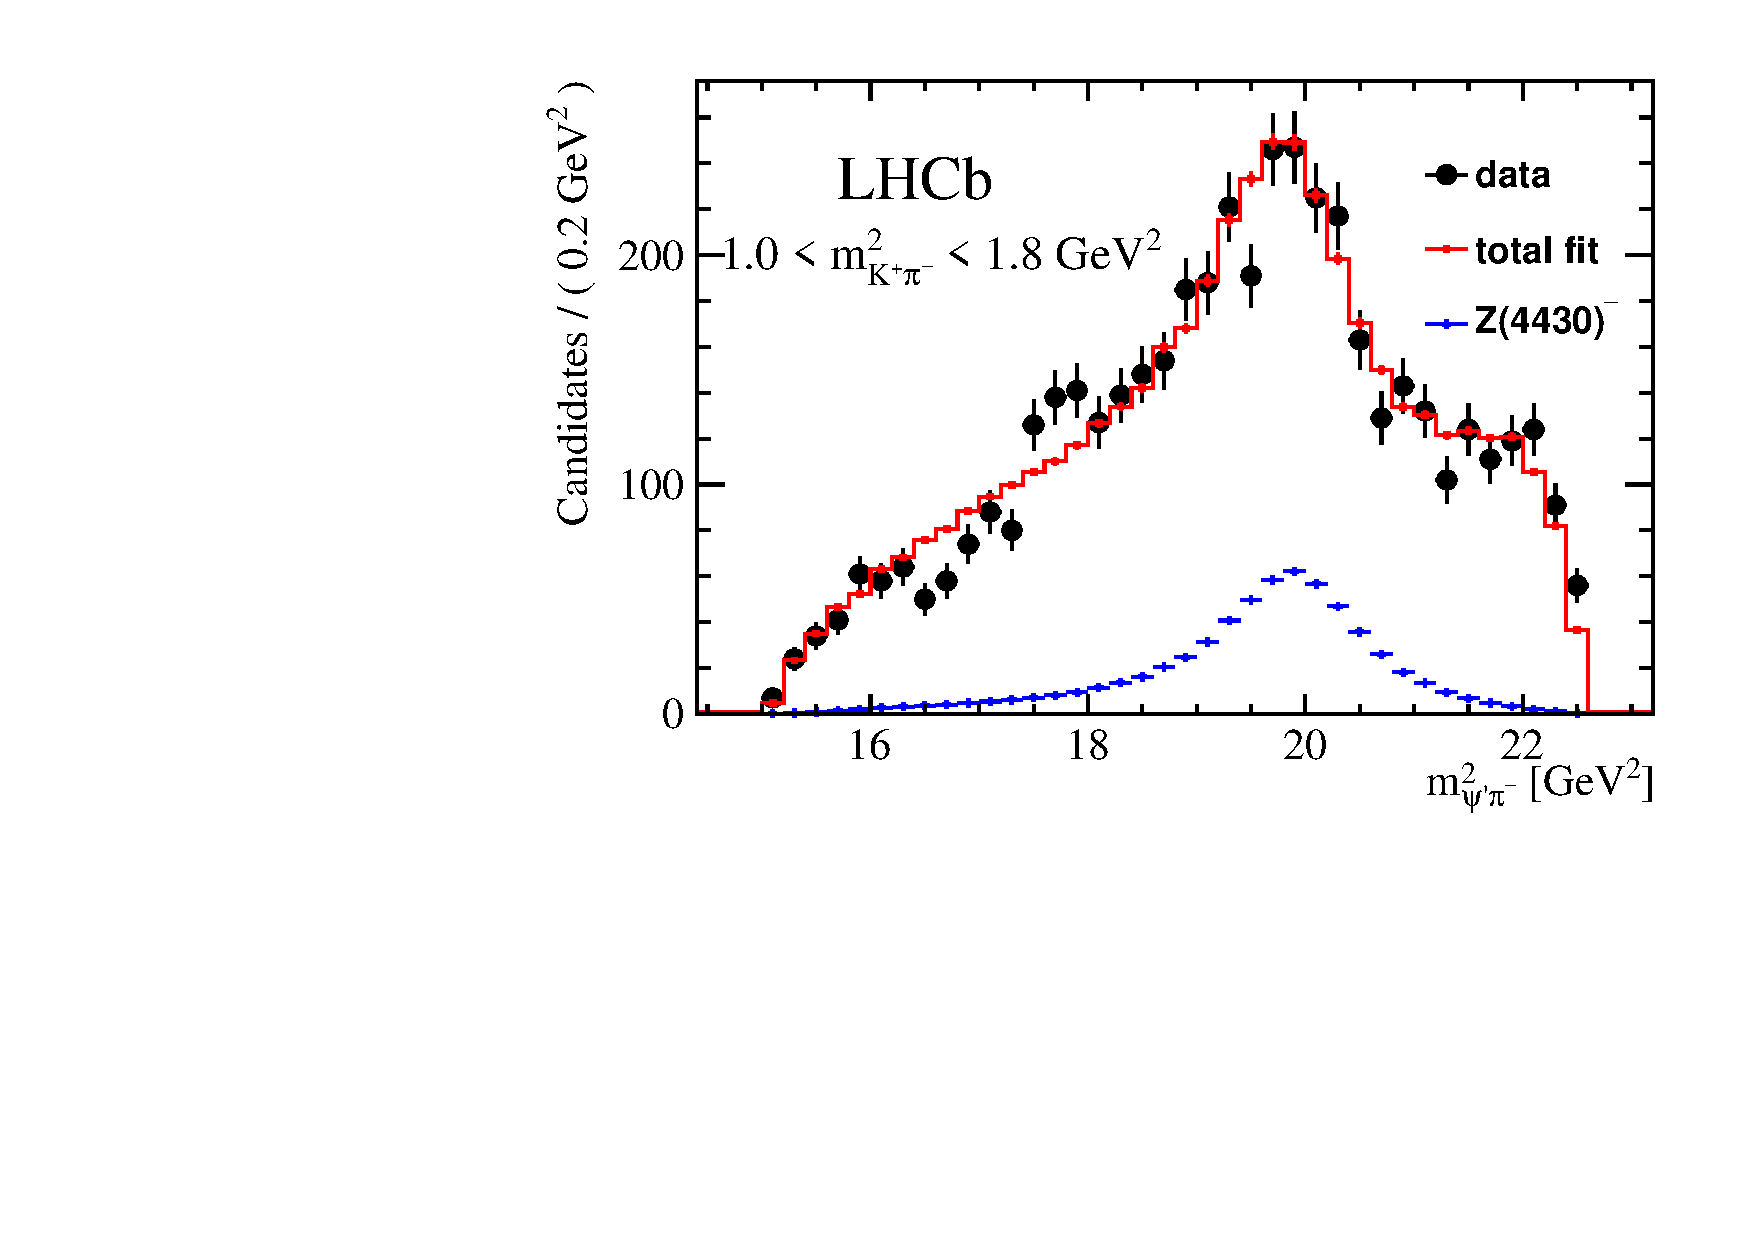
\includegraphics[width=1\linewidth]{../figures/Z4430_res.pdf}
          \end{center}
        \end{column}
        \begin{column}{.5\linewidth}
          \begin{center}
            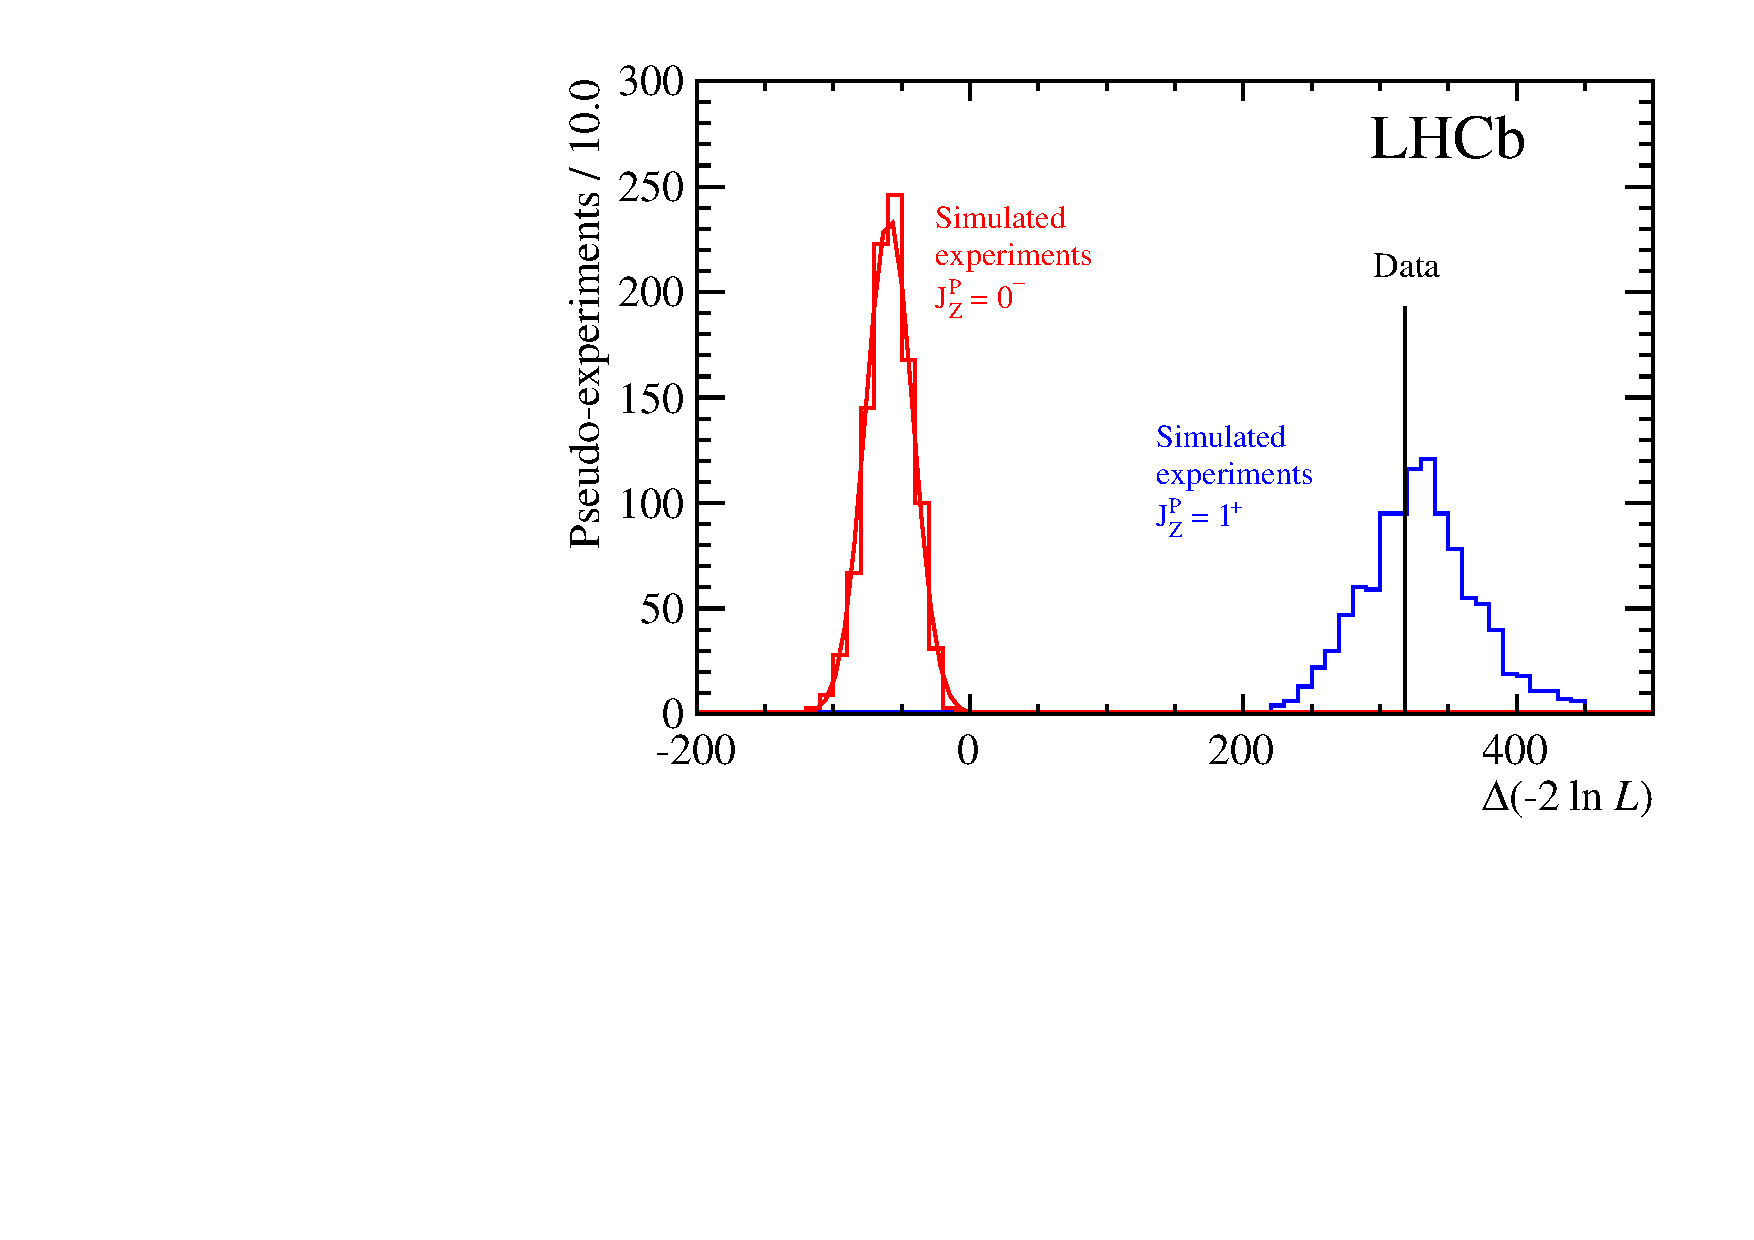
\includegraphics[width=1\linewidth]{../figures/Z4430_jp.pdf}
          \end{center}          
        \end{column}
      \end{columns}
    \end{center}
  }
  \tiny{Figures from: \url{http://cds.cern.ch/record/1693968}}
\end{frame}

\begin{frame}
  \frametitle{Summary}
  \begin{itemize}
  \item We've discussed some mesons beyond \su3flavor \qqbar.
  \item Hybrids, Glueballs, and Tetraquarks are all Lattice QCD allowed states beyond the non-relativistic quark model
  \item Experimental evidence exists for non $q\overline{q}$ mesons, supporting non-perturbative QCD.
  \item This includes the exotic pions we discussed and the $Z(4430)$, a confirmed tetraquark.
  \end{itemize}
\end{frame}

\begin{thebibliography}{9}
  % \bibitem{Barnes}
  %   T. Barnes, \textit{Exotic Mesons, Theory and Experiment}, arXiv:hep-ph/0007296, \url{http://arxiv.org/abs/hep-ph/0007296}
\bibitem{ketzer}
  Bernhard Ketzer, \textit{Hybrid Mesons}, Proceedings of Science, Sixth International Conference on Quarks and Nuclear Physics, PoS(QNP2012)025, \url{http://pos.sissa.it/archive/conferences/157/025/QNP2012_025.pdf} %\url{http://arxiv.org/abs/1208.5125}
  % \bibitem{Olsen}
  %   Stephen Lars Olsen, \textit{QCD exotics}, Hyperfine Interactions, \textbf{229}, \url{http://dx.doi.org/10.1007/s10751-014-1061-4}
\bibitem{belle}
  S.~K.~Choi~\emph{et. al.}, \emph{Observation of a Resonancelike Structure in the} $\pi^{+-}\psi^{\prime}$ \emph{Mass Distribution in Exclusive} $B\rightarrow K \pi^{+-}\psi^{\prime}$ \emph{Decays}. Phys. Rev. Lett. \textbf{100}, 142001 8 April 2008.
\bibitem{z4430_dmolecule}
  E.~Braaten~and~M.~Lu, \emph{Line shapes of the Z(4430)} Phys. Rev. D \textbf{79} 051503(R) 11 March 2009
\bibitem{lhcb} % {j4}
  LHCb Collaboration, R. Aaij \textit{et al.}, \textit{Observation of the Resonant Character of the }$Z(4430{)}^{-}$\textit{ State}, Phys. Rev. Lett., \textbf{112}, 22 (2014). \url{http://dx.doi.org/10.1103/PhysRevLett.112.222002}%\url{http://link.aps.org/doi/10.1103/PhysRevLett.112.222002}

\bibitem{j1}
  K.A. Olive \textit{et al.} (Particle Data Group), \textit{Non--\qqbar~Mesons} (Revised March 2006 by C. Amsler), Chin. Phys. C, 38, 090001 (2014), \url{http://pdg.lbl.gov/2006/reviews/nonqqbar_mxxx050.pdf}
\bibitem{j2}
  Vincent Mathieu, Nikolai Kochelev, and Vicente Vento, \emph{The Physics of Glueballs}, Int. J. Mod. Phys. E \textbf{18}, 1 (2009), \url{http://www.worldscientific.com/doi/abs/10.1142/S0218301309012124}
\bibitem{j3}
  Wolfgang Ochs, \emph{The status of glueballs}, J. Phys. G: Nucl. Part. Phys. \textbf{40}, 043001 (2013), \url{http://dx.doi.org/10.1088/0954-3899/40/4/043001}

\end{thebibliography}
\end{document}

